
\section{Matchings und alternierende Wege}

%\newcommand{\bc}{\bar{c}}

Ungerichteter Graph $G=(V,E)$\\
Definitionen:
\begin{description}
\item[Matching $M \subseteq E$] Jeder Knoten in $V$ ist inzident mit
höchstens einer Kante in $M$.
\item[$M$ überdeckt $v\in V$]
$(\exists e \in M) \; v$ inzident $e$\\
sonst ist $v$ {\em $M$-exponiert}.
Anzahl überdeckter Knoten: $2|M|$\\
Anzahl der exponierten Knoten: $|V| - 2|M|$\\
$\nu(G)$: Kardinalität eines maximum Matchings\\
$def(G)$: Minimum Anzahl exponierter Knoten
\[def(G) = |V| - 2 \nu(G) \; \; \mbox{"`Defizit"'}\]
\item[Perfektes Matching] Matching $M \subseteq E$ das alle Knoten in $V$
überdeckt.
\end{description}

Probleme:
\begin{itemize}
\item Hat $G$ ein perfektes Matching?
\item Finde ein maximum Matching in $G$
\item Finde ein perf. Matching mit Minimum Gewicht in $G$ mit
Kantengewichten.
\end{itemize}

Wenn $G$ bipartit: Max. Matching $\rightarrow$ ganzzahliges
Max-Fluss-Problem

$\left.\begin{array}{l}\mbox{min. Gewicht}\\\mbox{perf. Matching}\end{array}
\right\} \rightarrow$ Min-Kosten-Flussproblem (Übungsaufgabe 35)


Weitere Definitionen:
\begin{description}
\item[M-alternierender Weg] abwechselnd Kanten $e \in M$ und $e \notin M$
\item[M-augmentierender (-erhöhender) Weg] \mbox{}

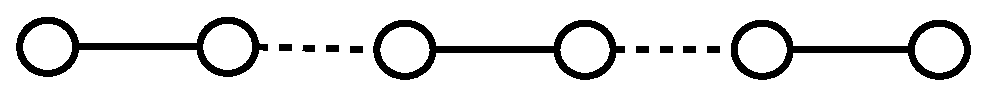
\includegraphics[width=5cm]{bilder/5-1augmWeg} \hspace{5mm} Konvention:
\begin{tabular}[c]{l}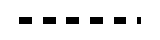
\includegraphics[width=0.6cm]{bilder/5-1augmWegKonv1}
$e \in M$\\

\includegraphics[width=0.6cm]{bilder/5-1augmWegKonv2} $e \notin M$
\end{tabular}

ist ein M-alternierender Weg dessen Endknoten $M$-exponiert sind.
\end{description}
Für $G$ bipartit:\\
$M$-augmentierender Weg $\leftrightarrow$ $x$ augmentierender Weg in der
Max-Fluss-Formulierung.\\
$\stackrel{\mbox{Kap. 3}}{\Rightarrow}$ $M$ Maximum $\leftrightarrow
\nexists$  augmentierender Weg

\begin{satz}
(nach Berge [1957]) Ein Matching in $G$ ist maximum genau dann, wenn kein
$M$-augmentierender Weg existiert.
\end{satz}
Beweis:
\begin{itemize}
\item["`$\Rightarrow$"'] $\exists$ $M$-augmentierender Weg $P$\\
$\Rightarrow M \; \Delta \; E(P)$ überdeckt 2 Knoten mehr ($\Delta$ steht
für symetrische Differenz, "`Drehe Kanten um"')\\
$\Rightarrow M$ ist nicht maximum
\item["`$\Leftarrow$"'] $M$ ist nicht maximum\\
$\Rightarrow \exists$ Matching $N$ mit $|N| > |M|$\\
$J:= N \Delta M$

Beispiel:

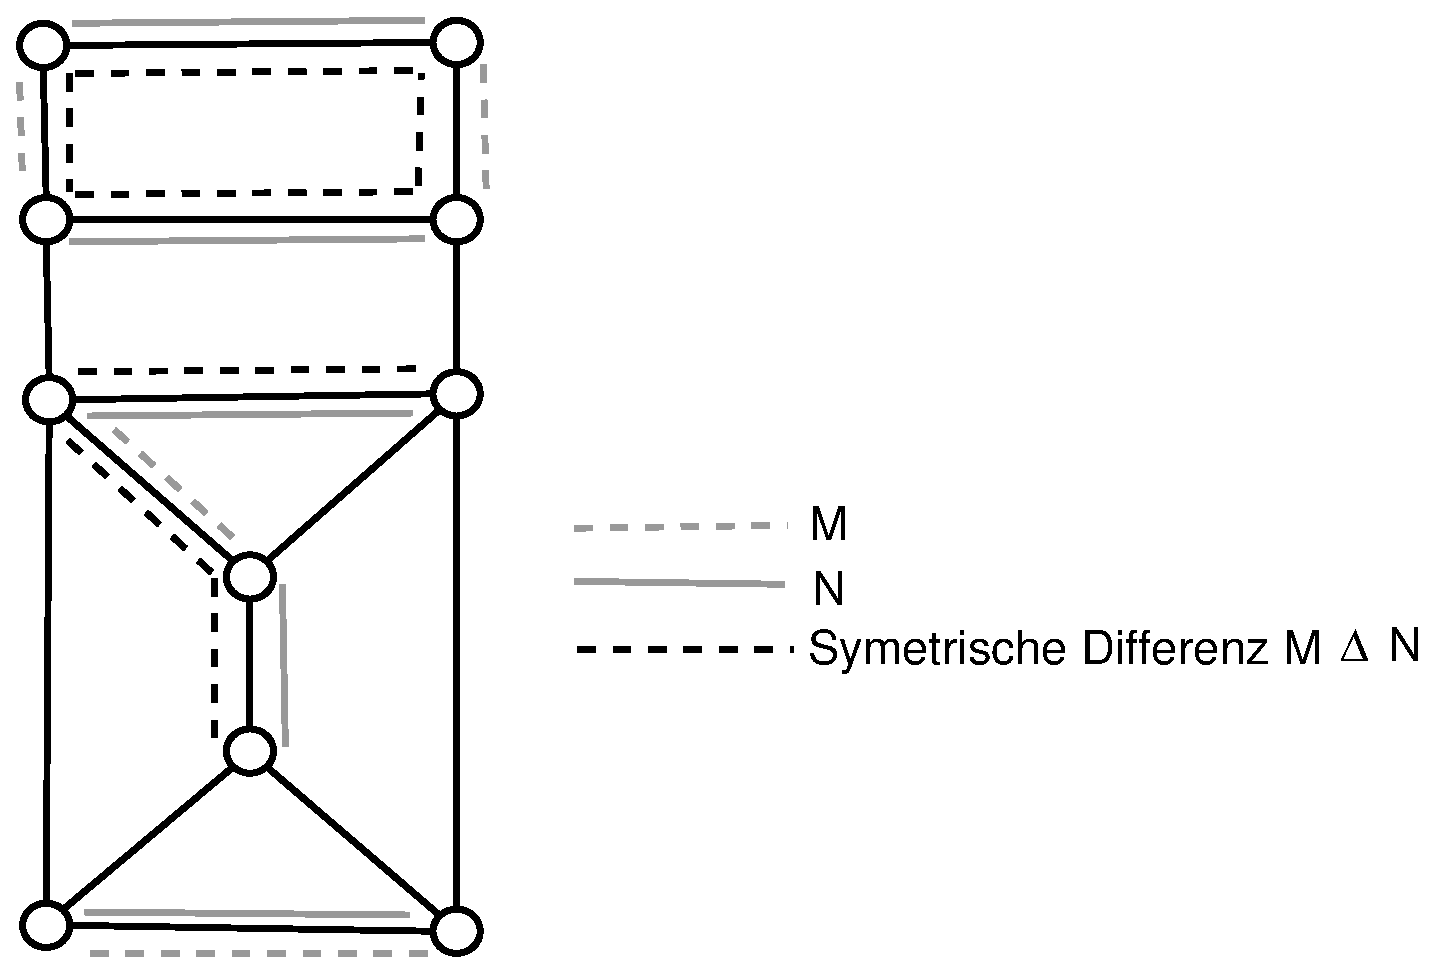
\includegraphics[height=5cm]{bilder/5-1DiffMatch}

$J:$ Knotendisjunkte alternierende Wege und alternierende Kreise gerader
Kardinalität.\\
$|N| > |M| \Rightarrow$ Ein Weg (von allen) in $J$ hat mehr $N$-Kanten als
$M$-Kanten. Dieser ist ein $M$-augmentierender Weg. q.e.d.

\end{itemize}

\paragraph{ungerade Kreise:}\mbox{}\\
Knotenüberdeckung: $A \subseteq V$ mit: Jede Kante hat wenigstens einen
Endknoten in $A$, also gilt:
\[\mbox{Kardinalität einer Knotenüberdeckung} \geqq \mbox{Kardinalität eines
Matchings}\] 

{\bf Satz} von König (Aufgabe 24)
\[\begin{array}{rcl}
\mbox{Wenn $G$ bipartit} &\Rightarrow& (\exists \mbox{ Knotenüberdeckung }
A)\\
&& ( \exists \mbox{ Matching } M)\\
&&|A| = | M|
\end{array}
\]
Das gilt {\em nicht} allgemein, so z.B. nicht in ungeraden kreisen wie dem
folgenden mit der Länge $k+1$ (Eine
minimale Knotenüberdeckung $A$ ist durch die grauen Kreise, ein 
maximales Matching $M$ durch die gestrichelten Linien angedeutet):

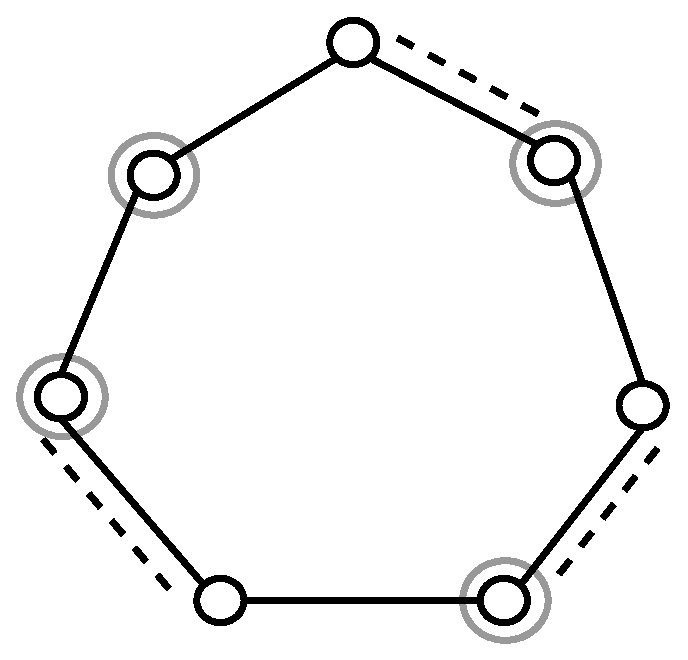
\includegraphics[height=4cm]{bilder/5-1UngerKreis}

Hier gilt offensichtlich $|M| \leqq k$ und $|A| \geqq k+1$. Wir suchen nun
eine bessere Schranke:

Sei $A\subseteq V$ mit $G\wout A$ (Knoten $A$ gelöscht hat $k$ Komponenten
$h_1, h_2,\ldots,h_k$ mit $|V(H_i)|$ ungerade. 

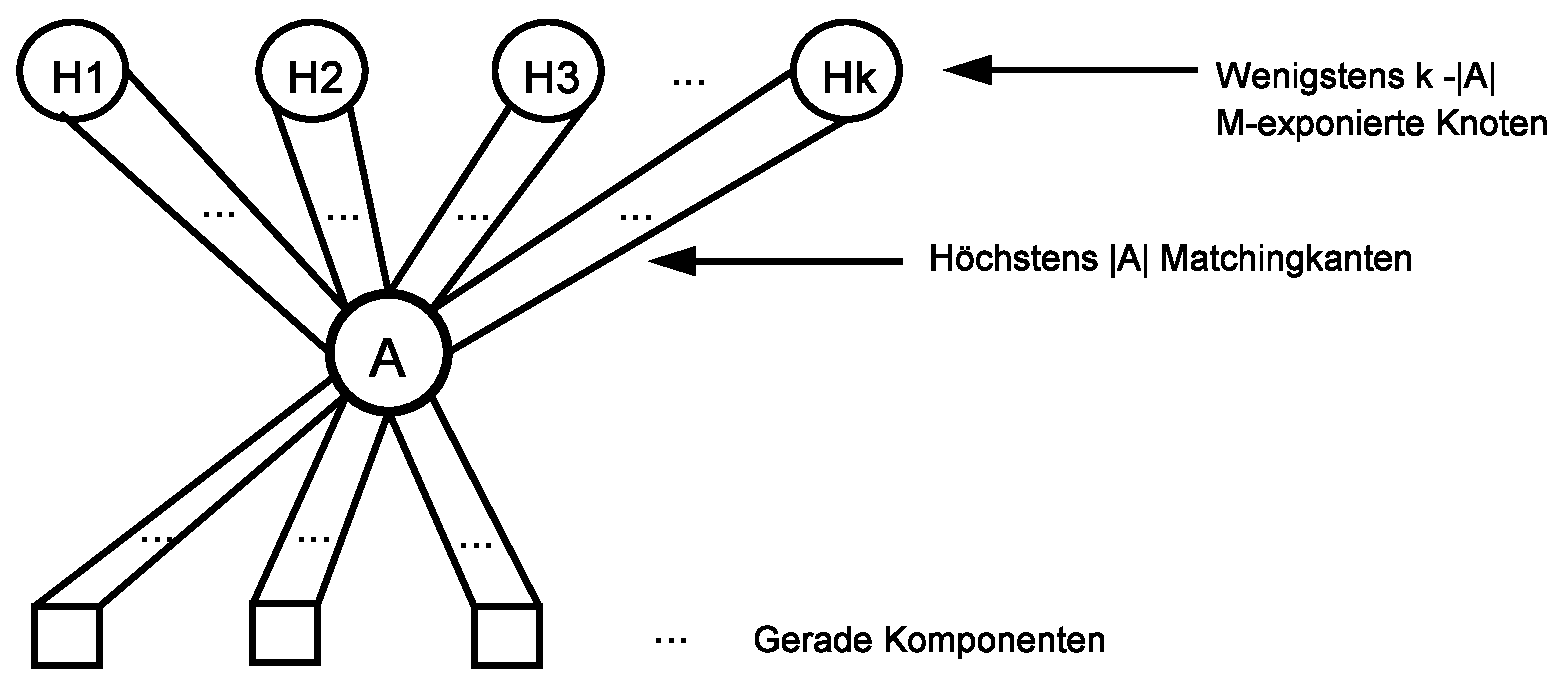
\includegraphics[height=5cm]{bilder/5-1ARausgenommen}

Nun definieren wir $OC(G) := $ Anzahl ungerader Komponenten von $G$, z.B.:

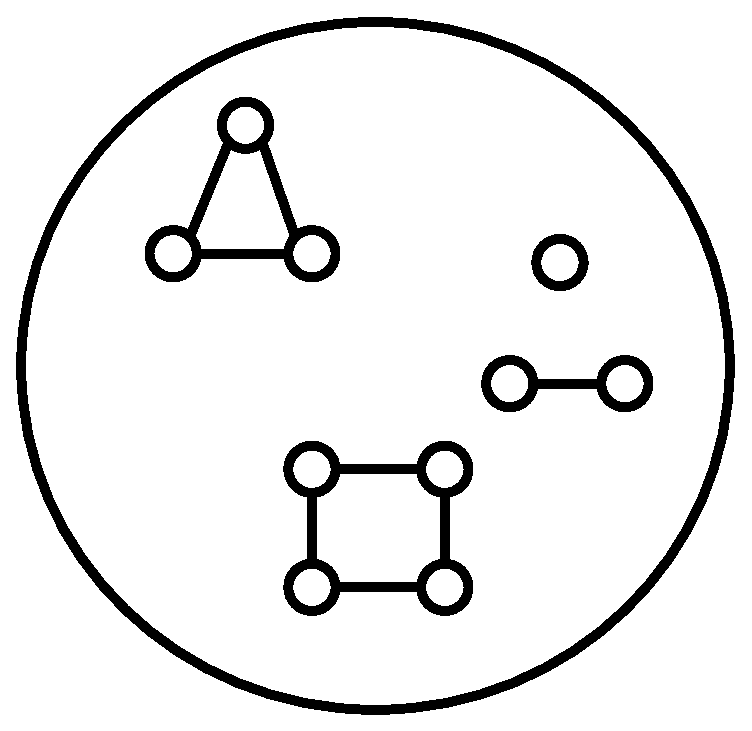
\includegraphics[height=3cm]{bilder/5-1AnzUngKomp} \hspace{5mm} $OC(G)=2$

Also $(\forall A \subseteq V)$:
\[\nu(G) = \frac{1}{2} (|V| - OC(G\wout A) + |A|)\]
Falls $A$ Knotenüberdeckung ist:\\
$|V| -|A|$ ungerade Komponenten in $G\wout A$ (einzelne Knoten)\\
$\Rightarrow \nu(G) \leqq \frac{1}{2} (|V| - (|V| - |A|) + |A|) = |A|$

Spezialfall, d.h. die untere Schranke ist wenigstens so gut wie die
Überdeckungsschranke, sogar besser:

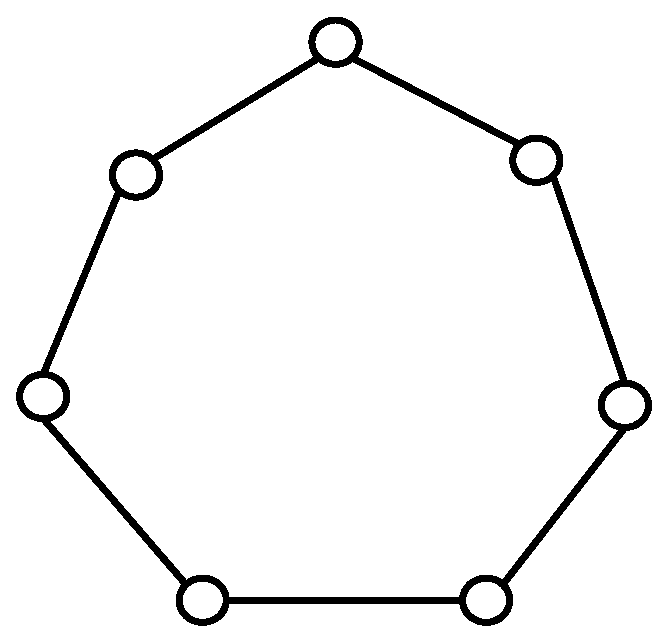
\includegraphics[height=3cm]{bilder/5-1UngerKreis2}\hspace{5mm} 
\parbox[b]{10cm}{Ungerader Kreis der
Länge $2k+1$\\$A = \varnothing$: $\nu(G) \leqq \frac{1}{2}(|V|-1) = k$\\
(bisher nur $k+1$, also besser!)}

Für jedes $A\subseteq V$ heißt die vorhin bewiesene Schranke für
Kardinalität eines Matchings:

\[\nu(G) \leqq \frac{1}{2}(|V| - OC(G\wout A) + |A|)\]

Dies ist die "`Tutte-Berge-Schranke"'. Es folgt sofort die sog. "`Tutte
Bedingung"':\\
Hat $G=(V,E)$ ein perfektes Matching, so gilt für jede Teilmenge $A
\subseteq V$: $OC(G\wout A) \leqq |A|$

Wir werden später sehen, dass die Tutte Berge Schranke angenommen wird und
die Tutte-Bedingung auch hinreichend ist.

\section{Maximum Matching}
Zunächst suche nach perfektem Matching (danach max. Matching)

\paragraph{Alternierende Bäume} \mbox{}\\
$G = (V,E)$, $M \subseteq E$ Matching, $r$ ein $M$-exponierter Knoten,
$M$-alternierender Baum $T$:

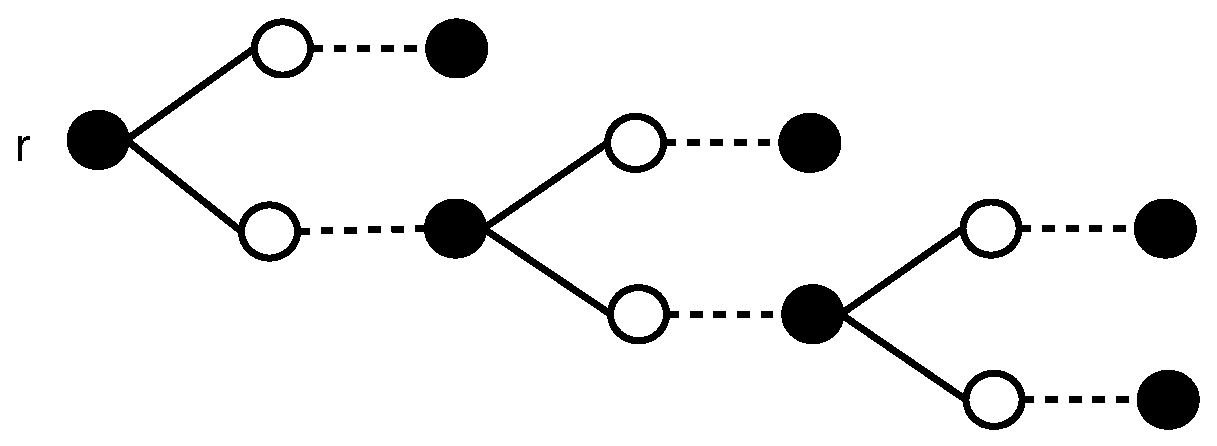
\includegraphics[height=2.5cm]{bilder/5-2altBaum}

$A(T)=\{v \in V(T)| v \mbox{ hat ungerade Distanz von }r\}$ "`ungerade
Knoten"' $\circ$\\
$B(T)=\{v \in V(T)| v \mbox{ hat gerade Distanz von }r\}$ "`gerade Knoten
"' $\bullet$

Eigenschaften:
\begin{itemize}
\item Jedes $v \in V(T) \wout \{r\}$ wird von einer Kante $e \in M(T)$
überdeckt.
\item Für jedes $v\in V(T)$ ist der $(r,v)$-Weg in $T$ $M$-alternierend.
\item $|B(T)| = |A(T)| +1$
\end{itemize}

Zum Anfang der Vorlesung legte Prof. Jünger einen Beispielgraph auf:

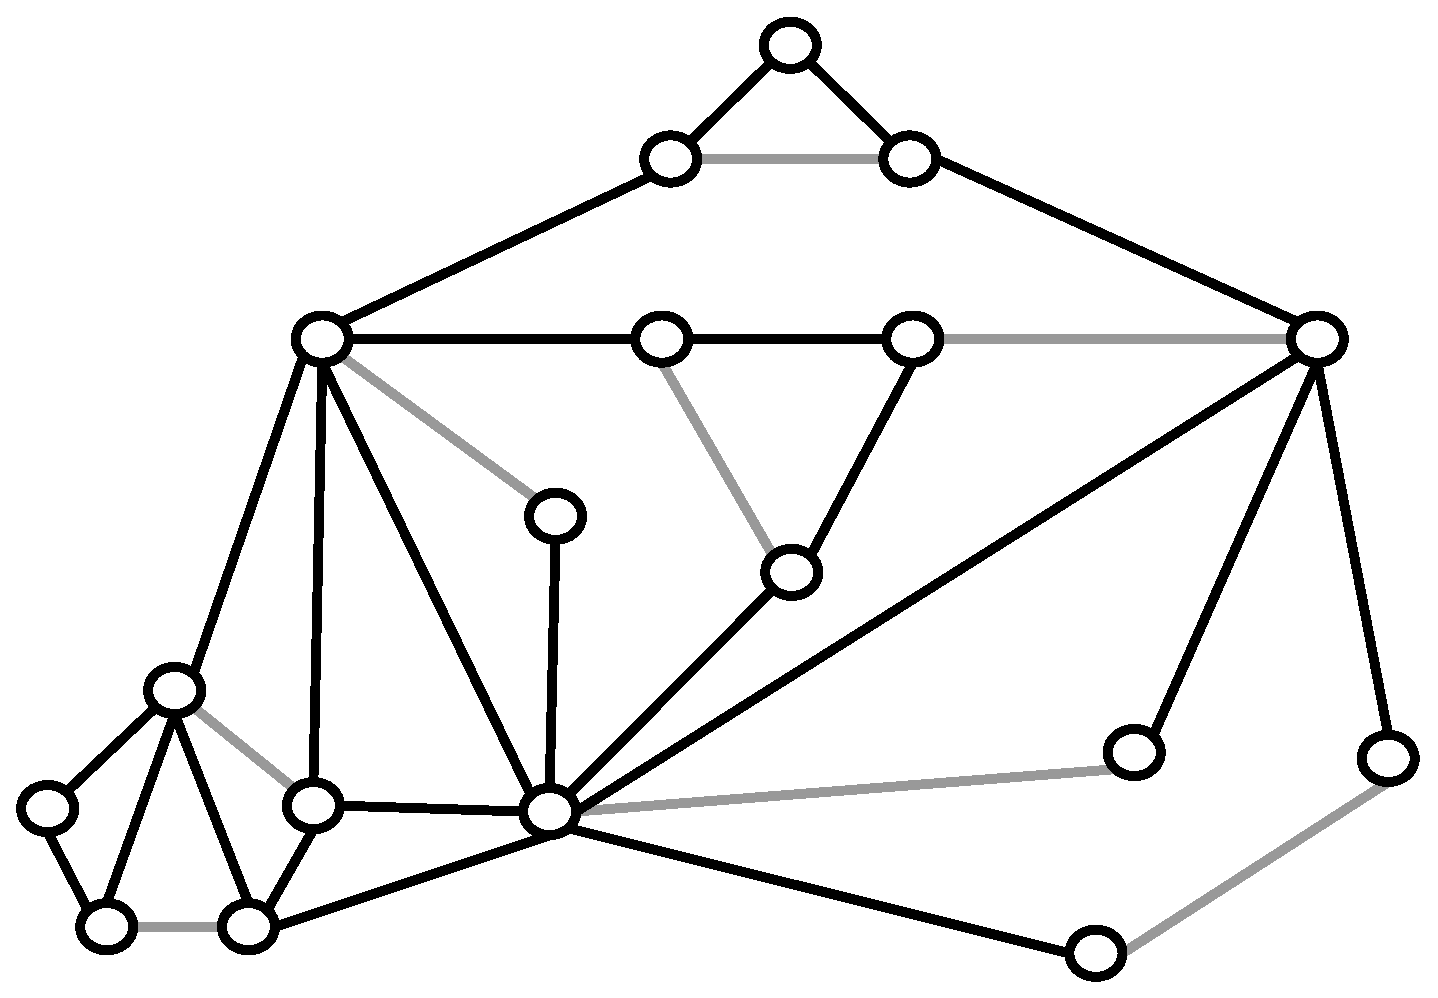
\includegraphics[height=4cm]{bilder/5-2altBaum2}

$G=(V,E)$\\
$|V| = 18$\\
$|M| = 8$, d.h. zwei exponierte Knoten\\

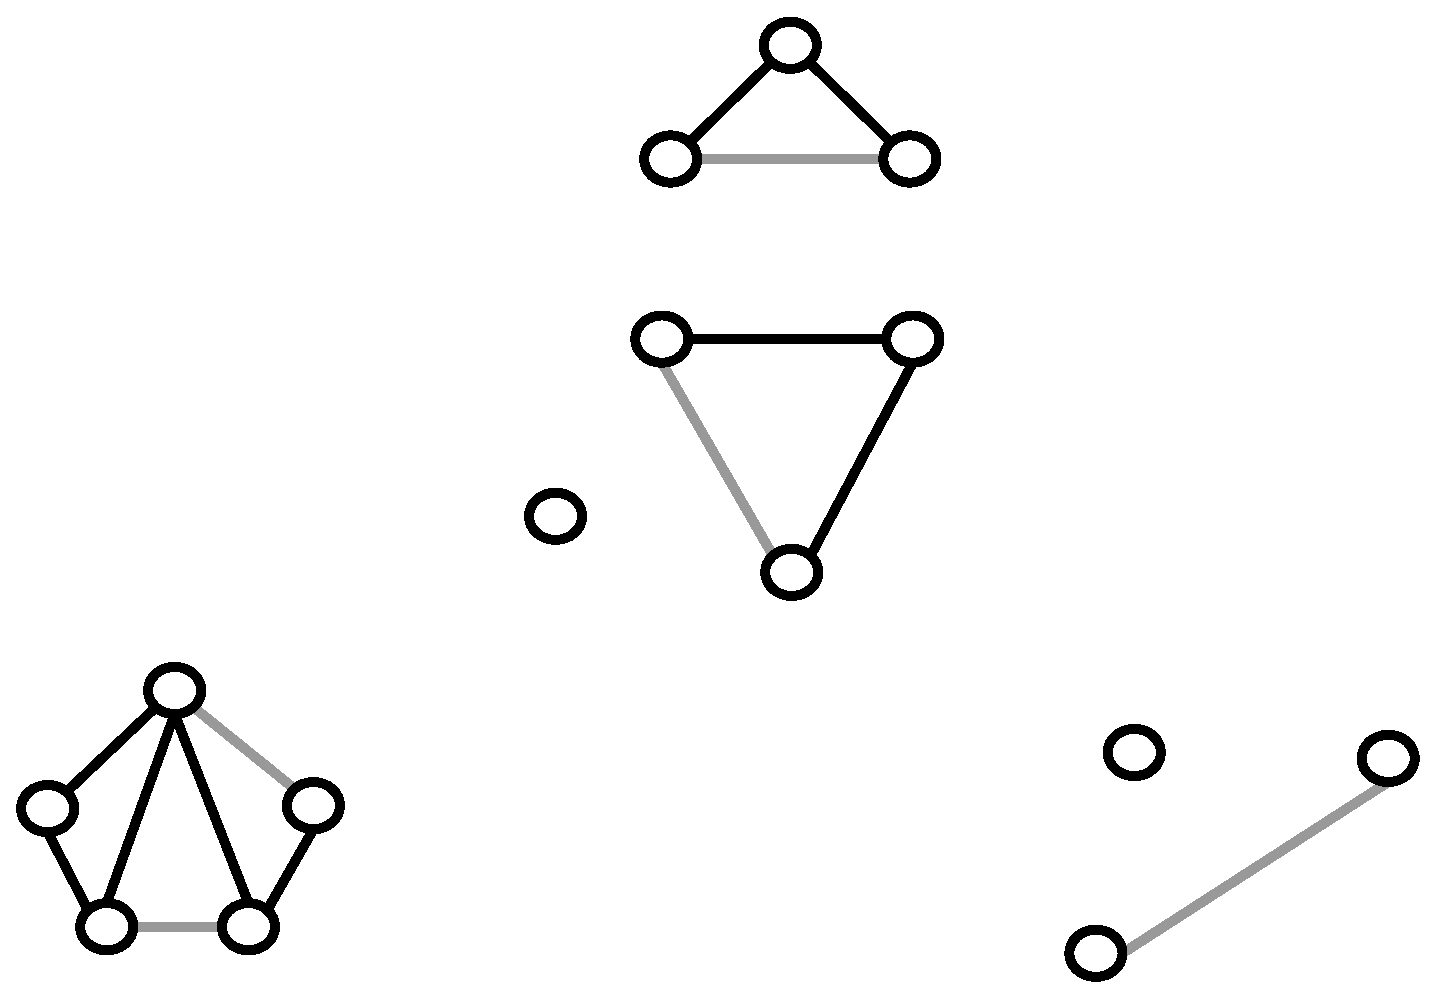
\includegraphics[height=4cm]{bilder/5-2altBaum3}

$OC(G\wout A) = 5$\\
$\stackrel{\mbox{\scriptsize TB-Formel}}{\Rightarrow} \nu(G) \leqq
\frac{1}{2}(18-5+3)=8$\\
$\Rightarrow M$ Matching max. Kardinalität.

\subsubsection{"`Unterprogramme"}
\paragraph{Benutze $v w$ zur Baumerweiterung} \mbox{}\\
Eingabe: Matching $M'$ von $G'$, $M'$ alternierender Baum $T$, $v w \in
E(G')$ mit $v \in B(T)$, $w\notin V(T)$, $w \; M'$-überdeckt.

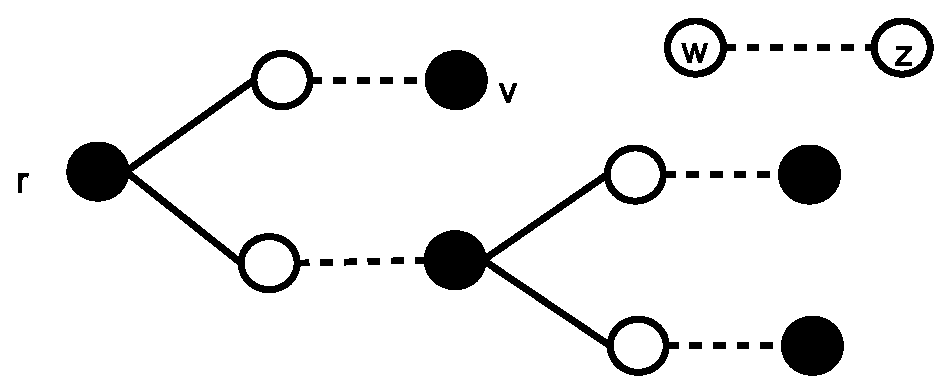
\includegraphics[height=2cm]{bilder/5-2vwBaumerw}

Aktion: Sei $w z$ die überdeckende Kante in $M'$\\
$T \leftarrow (V(T) \cup\{w,z\},\; E(T) \cup \{v w, w z\})$

\paragraph{Benutze $v w$ zur $M'$-Augmentierung} \mbox{}\\
Eingabe: Matching $M'$ von $G'$, $M'$ alternierender Baum $T$ mit Wurzel $r$, $v w\in
E(G')$ mit $v \in B(T)$, $w\notin V(T)$, $w$ $M'$-exponiert.

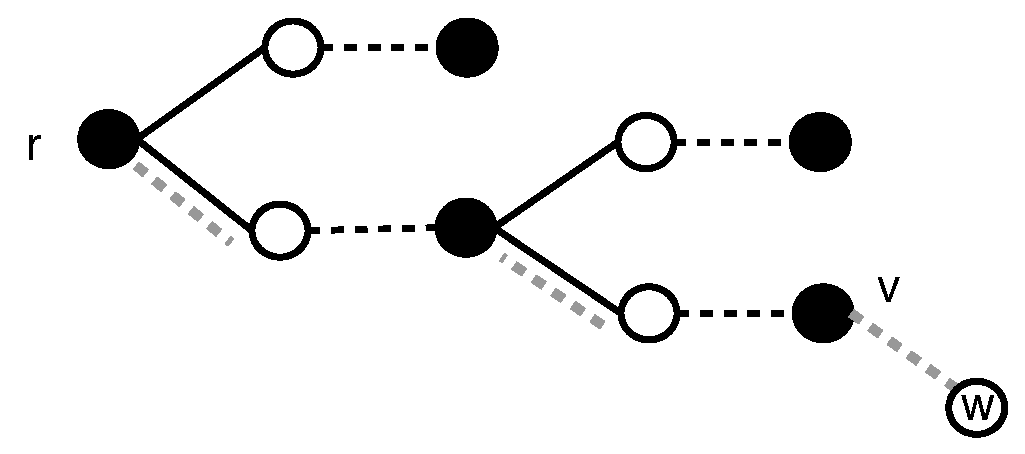
\includegraphics[height=2cm]{bilder/5-2vwAugment}

Aktion: Sei $P$ der $(r,v)$-Weg in $T \cup \{v w\}$\\
$M' \leftarrow M' \; \Delta \; E(P)$

Ein $M$-alternierender Baum $T$ in $G$ ist {\em frustriert} falls jede
Kante in $E(G)$ mit einem Ende in $B(T)$ das andere Ende in $A(T)$ hat.

\begin{lemma} \label{FrustKeinMatch}
Hat $G$ ein Matching $M$ und einen frustrierten $M$-alternierenden Baum
$T$, so hat $G$ kein perfektes Matching.
\end{lemma}
Beweis: $\forall v \in B(T)$ ist $\{v\}$ ungerade Komponente von $G\wout
A(T)$, d.h. für $A=A(T) \subseteq V$ gilt:\\
$OC(G\wout A) \geqq |B(T)| > |A(T)| = |A|$\\
$\stackrel{\mbox{\scriptsize Tutte-Bed.}}{\Rightarrow} G$ hat kein perf. Matching. 
\subsubsection{Der Bipartite Fall}

Perf. Matching Algorithmus für bipartite Graphen
\begin{algorithmic}
\STATE $M \leftarrow \varnothing$;
\STATE $T \leftarrow (\{r\}, \varnothing)$; ($r$ beliebig)
\WHILE{($\exists v w \in E$ mit $v \in B(T)$, $w\not\in V(T)$)}
\IF{($w$ ist $M$-exponiert)}
\STATE Benutze $v w$ zur $M$-Augmentierung;
\IF{($\nexists$ $M$-exponierter Knoten in $G$)}
\STATE STOP "`$M$ ist perfektes Matching"';
\ELSE 
\STATE $T:=(\{r\},\varnothing)$ wobei $r$ $M$-exponierter Knoten;
\ENDIF
\ELSE 
\STATE Benutze $v w$ zur Baumerweiterung;
\ENDIF
\ENDWHILE
\STATE STOP "`$G$ hat kein perf. Matching"';
\end{algorithmic}

\begin{lemma}
Ist in obigem Algorithmus die while-Bedingung nicht erfüllt, so hat $G$
kein perf. Matching.
\end{lemma}
Beweis: Wir zeigen $T$ ist frustriert ($\stackrel{\mbox{\scriptsize
\ref{FrustKeinMatch}}}{\Rightarrow} \nexists$ perf. Matching)\\
$\nexists v w \in E \mbox{ mit } v \in B(T)$, $w \not\in V(T)$\\
$\Rightarrow (\forall v w  \in E \mbox{ mit } v \in B(T)) \; w \in A(T)$
oder $w \in B(T)$

Annahme $w \in B(T)$

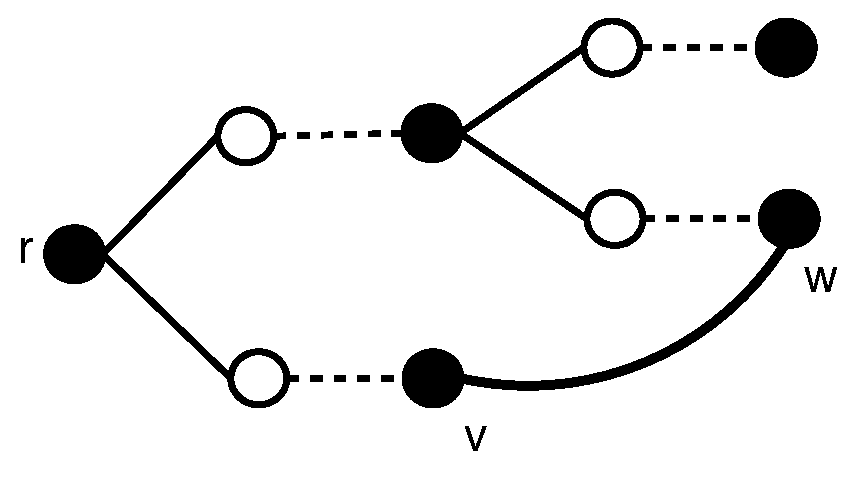
\includegraphics[height=2cm]{bilder/5-2BewL5-3}

$\Rightarrow G$ hat ungeraden Kreis\\
$=G$ ist nicht bipartit $\lightning$ 
$\Rightarrow T$ ist frustriert $\stackrel{\mbox{\scriptsize
\ref{FrustKeinMatch}}}{\Rightarrow}G$ hat kein perf. Matching. q.e.d.

\paragraph{Schrumpfen ungerader Kreise}\mbox{}\\
$C$ ungerader Kreis in $G$.\\
$G':= G \times C$: Subgraph von $G$ der durch das Schrumpfen des Kreises
$C$ entsteht.

$V(G') =(V\wout V(C)) \cup c$ ($c$ ist neuer Knoten statt Kreis)\\
$E(G') = E \wout \gamma(V(C))$ mit Endknoten in $V(G)$ ersetzt durch
$c$.\\
Bsp:

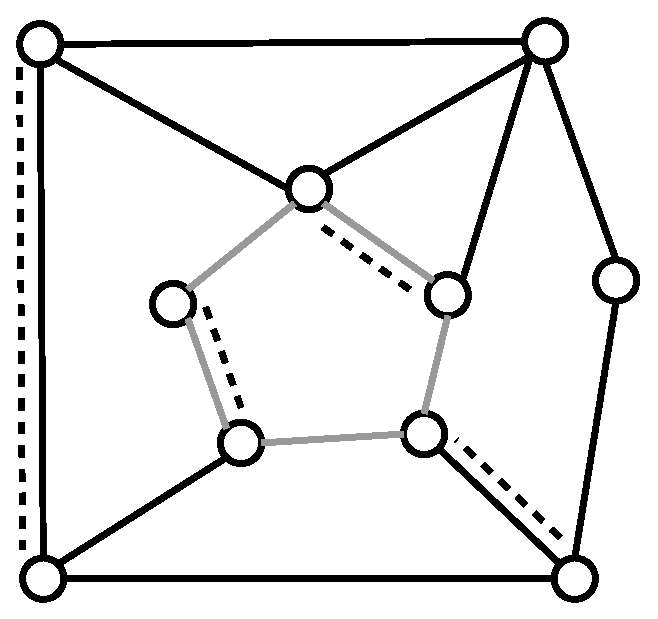
\includegraphics[height=3cm]{bilder/5-2Schrumpfb}
\hspace{4mm}$\rightarrow$\hspace{4mm}
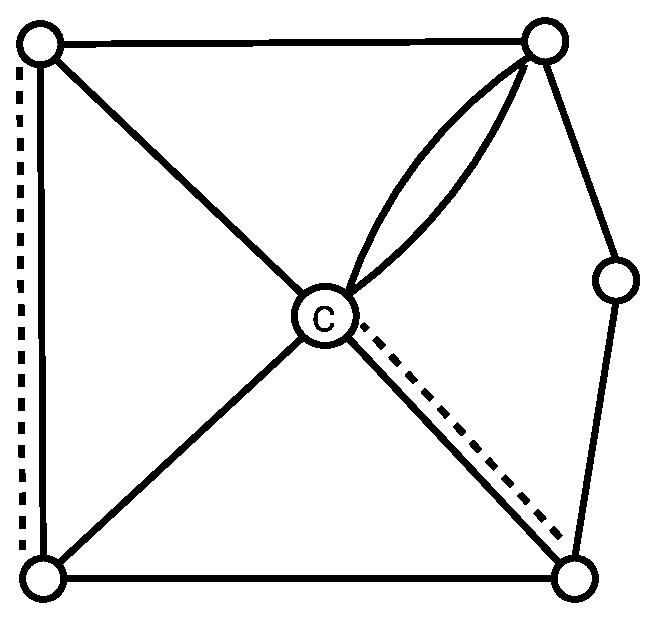
\includegraphics[height=3cm]{bilder/5-2Schrumpfb2}

Die Matchingkanten sind durch die gestrichelten Linien angedeutet.

\begin{lemma}
Sei $C$ ein ungerader Kreis in $G$, $G' = G \times C$ und $M'$ ein Matching
in $G'$. Dann existiert ein Matching $M$ in $G$ mit $M\subseteq M' \cup
E(C)$ und die Anzahl $M$-exponierter Knoten in $G$ ist dieselbe wie die
der $M$-exponierten Knoten in $G'$.
\end{lemma}

D.h. $\nu(G) \geqq \nu(G \times C) + \frac{|V(C)|-1}{2}$\\
b.z.w.: $def(G) \leqq def(G\times C)$

\subsubsection{Der Blütenschrumpfalgorithmus}

Im Original: "blossom shrinking"' für perf. Matching von Jack Edmonds, Name
des Papers: "`Paths, Trees and Flowers"'.

Aus $G$ entsteht durch wiederholtes Schrumpfen ungerader Kreise $G'$. $G'$
hat also zum einen Orginalknoten von $G$ als auch Pseudoknoten, die durch
Schrumpfen entstanden sind.

$v \in V(G')$: $S(v)$ Menge der zu $v$ gehörigen Originalknoten (rekursiv
ermittelt).\\
$|S(v)|$ ist immer ungerade ($S(v) = {v}$ für Originalknoten)\\
$\{ S(v) | v \in G' \}$ Partition von $V(G)$

Analogon zu Lemma \ref{FrustKeinMatch}:
\begin{lemma} \label{BSFrustKeinMatch}
Sei $G'$ von $G$ abgeleitet, $M'$ Matching in $G'$, $T$ ein
$M'$-alternierender Baum in G' und kein Pseudoknoten in $A(T)$. Ist $T$
frustriert, so hat $G$ kein perf. Matching
\end{lemma}
Beweis: Entfernung von $A(T)$ aus $V(G)$ ergibt für alle $v\in B(T)$
ungerade Komponenten mit Knotenmenge $S(v)$.\\
$\Rightarrow OC(G\wout A(T))\geqq |B(T)|> |A(T)|$\\
$\stackrel{\mbox{\scriptsize Tutte Bed.}}{\Longrightarrow} G$ hat kein perf. 
Matching. q.e.d.

\begin{itemize}
\item Produziere abgeleitete Graphen $G'$
\item Perf. Matching in $G'\rightarrow$ perf. Matching in $G$
\item Gewisse frustrierte Bäume in $G' \rightarrow$ kein perf Matching 
\end{itemize}

Welche Kreise schrumpfen wir aber nun?

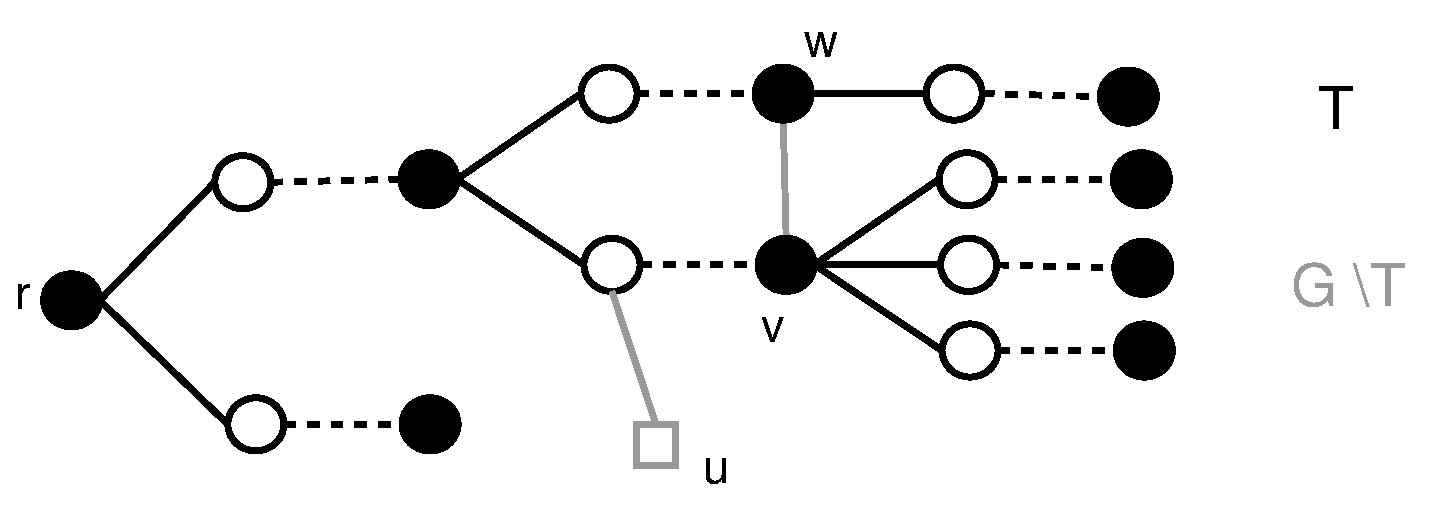
\includegraphics[height=3cm]{bilder/5-2Bluetenschr1}
\begin{itemize}
\item $M$ ist nicht optimal ($\exists$ perf. Matching!)
\item keine Erweiterung/Augmentierung möglich
\item $T$ nicht frustriert.
\end{itemize}
$vw$ erzeugt ungeraden Kreis "`Blüte"' (Edmonds)\\
Schrumpfen der Blüte.

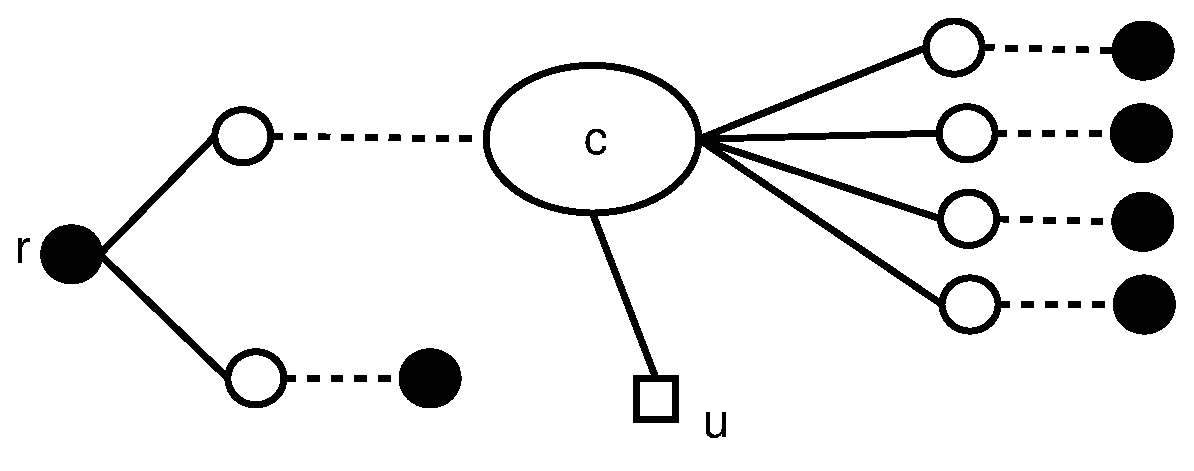
\includegraphics[height=3cm]{bilder/5-2Bluetenschr2}


Behalte $T$ und $M$, Augmentiere:

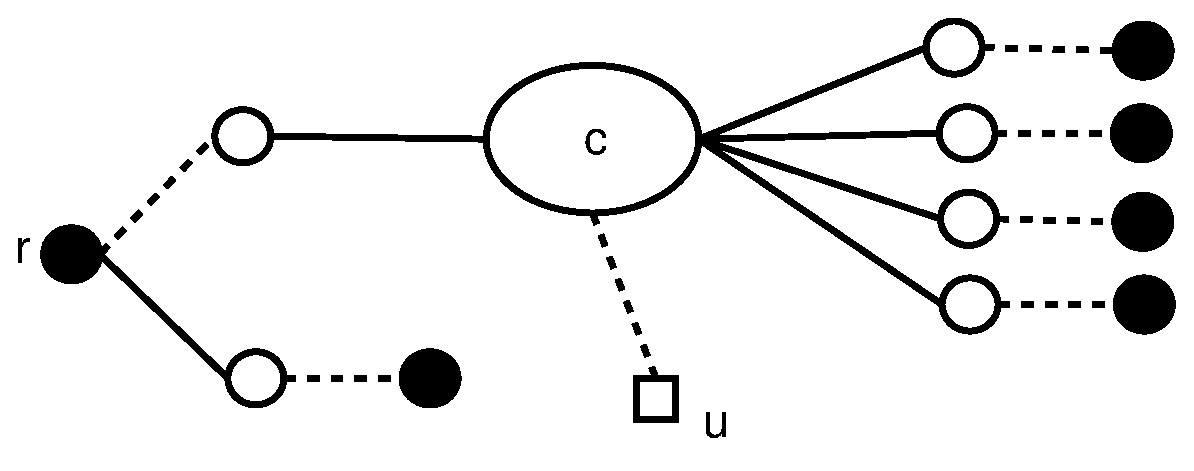
\includegraphics[height=3cm]{bilder/5-2Bluetenschr3}

Entschrumpfen:

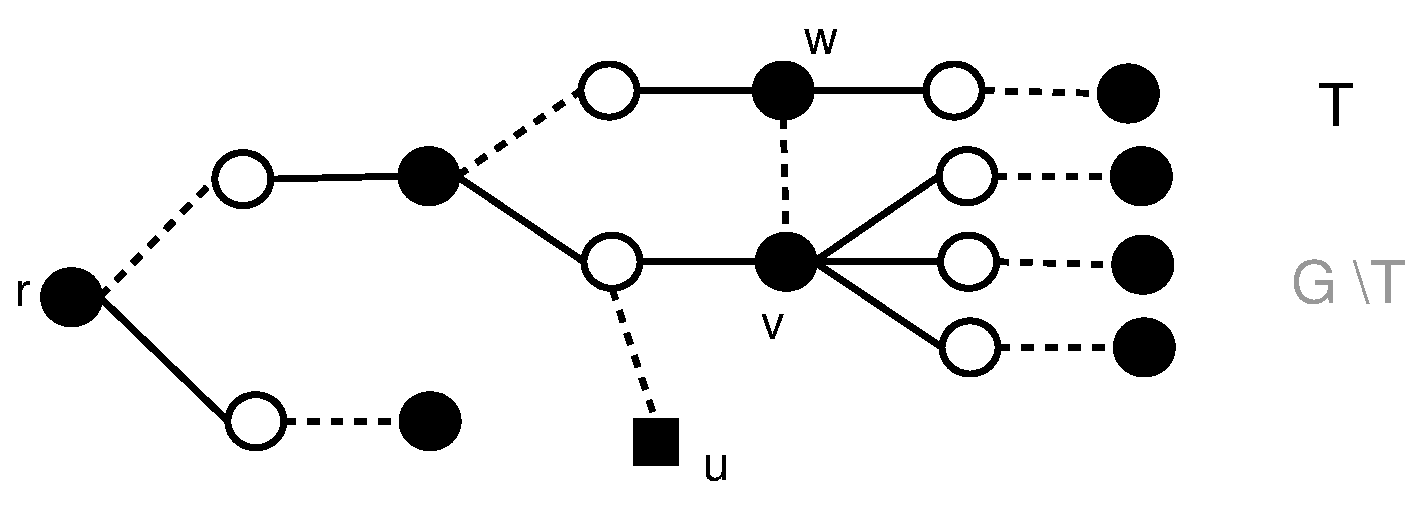
\includegraphics[height=3cm]{bilder/5-2Bluetenschr4}

\paragraph{Benutze $vw$ zum Schrumpfen und adaptiere $M'$ und $T$}
\mbox{}\\

Eingaben:
\begin{itemize}
\item Matching $M'$ von $G'$
\item $M'$-alternierenden Baum $T$
\item $vw \in E(G')$ mit $v,w \in B(T)$
\end{itemize}
Sei $C$ der Kreis gebildet aus $v w$ und dem $(v,w)$-Weg in $T$.

$G' \leftarrow G' \times C$;\\
$M' \leftarrow M' \wout E(C)$;\\
$E(T) \leftarrow E(T) \wout E(C)$;

\begin{lemma}
Nach Anwendung des obigen Unterprogramms "`Schrumpf"' ist $M'$ ein Matching
in $G'$, $T$ ein $M'$-alternierender Baum in $G'$ und $c\in B(T)$.
\end{lemma}
Beweis: Übungen :)

\paragraph{Blüten-Schrumpf-Algorithmus für perfektes Matching}\mbox{}\\
Eingabe: Graph $G$ und Matching $M$ in $G$


\begin{algorithmic}
%\newenvironment{ALC@case}{\begin{ALC@g}}{\end{ALC@g}}
%\newcommand{\CASE}[2][default]{\ALC@it\textbf{case}\ ##2\ %
%\ALC@com{##1}\begin{ALC@case}}
%\newcommand{\ENDCASE}{\end{ALC@case}}
\IF{($M$ ist perfekt)} 
\STATE STOP "`$M$ ist ein perfektes Matching"';
\ENDIF
\STATE $M' \leftarrow M$;
\STATE $G' \leftarrow G$;
\STATE Wähle $M'$-exponierten Knoten $r$ in $G'$;
\STATE $T \leftarrow (\{r\},\varnothing)$;
\WHILE{($\exists vw \in E'$ mit $v\in B(T)$, $w\notin A(T)$)}
\CASE{($w\notin V(T)$ und $w$ ist $M'$-exponiert)}
\STATE Benutze $vw$ zur $M'$-Augmentierung;
\STATE Erweitere $M'$ zu einem Matching $M$ von $G$;
\STATE $M' \leftarrow M$;
\STATE $G' \leftarrow G$;
\IF{($\nexists M'$-exponierter Knoten in $G'$)}
\STATE STOP "`$M'$ ist ein perfektes Matching"';
\ELSE 
\STATE $T \leftarrow (\{r\},\varnothing)$ wobei $r$ $M'$-exponiert ist;
\ENDIF
\ENDCASE
\CASE{($w \notin V(T)$ und $w$ ist $M'$-überdeckt)}
\STATE Benutze $vw$ zur Baumerweiterung;
\ENDCASE
\CASE{($w \in B(T)$)}
\STATE Benutze $vw$ zum Schrumpfen und adaptiere $M'$ und $T$;
\ENDCASE
\ENDWHILE
\STATE STOP "`$G$ hat kein perfektes Matching"';
\end{algorithmic}

\begin{satz}
Der Blütenschrumpf-Algorithmus terminiert nach:
$O(n)$ Augmentierungen\\
$O(n^2)$ Schrumpf-Schritten\\
$O(n^2)$ Baumerweiterungs-Schritten\\
Er entscheidet korrekt, ob $G$ ein perf. Matching hat.
\end{satz}
Beweis: $M'$ ist in jeder Iteration ein Matching, es gibt jedes mal weniger
exponierte Knoten $\Rightarrow O(n)$ Augmentierungen.

Jeder Schrumpf-Schritt:
\begin{itemize}
\item erniedrigt die Anzahl der Knoten in $G'$
\item erhält die Anzahl, der Nicht-Baumknoten
\end{itemize}
Jeder Baumerweiterungsschritt:
\begin{itemize}
\item erniedrigt die Anzahl der Nicht-Baumknoten
\item erhält die Anzahl der Knoten in $G'$
\end{itemize}
Zwischen den Augmentierungen höchstens $O(n)$
Schrumpf/Baumerweiterungsschritte\\
$\Rightarrow$ Insgesamt $O(n^2)$ Schrumpf/Baumerweiterungsschritte

Jedes $G'$ ist aus $G$ abgeleitet\\
Hält der Algorithmus mit "`$\nexists$ perf. Matching"'\\
$\Rightarrow \exists$ frustrierter Baum $T$ mit Voraussetzungen für Lemma  
\ref{BSFrustKeinMatch}\\
$\Rightarrow G$ hat kein perf. Matching q.e.d.

\paragraph{Der Blüten-Schrumpf Algorithmus für maximum Matching}

Der Blüten-Schrumpf Algorithmus für perf. Matching terminierte mit: STOP
"`$G$ hat kein perfektes Matching"'. Wir übernehmen $G'$, $M'$ und $T$ und
arbeiten wie folgt weiter:
\begin{algorithmic}
\STATE Entferne $V(T)$ aus $G'$;
\STATE Falls ein exponierter Knoten übrig ist: Anwendung des Blütenschrumpf
Algorithmus auf neues $G'$ ohne entfernte Kanten. (Neues $G'$ hat keine
Pseudoknoten.);
\STATE Wiederhole bis kein exponierte Knoten übrig bleibt;
\STATE Restauriere Original $G'$ mit allen produzierten Matchingkanten;
\STATE Bestimme korrespondierendes Matching in $G$
\end{algorithmic}

Seien $T_1, T_2, T_3 \ldots T_k$ die generierten frustrierten Bäume\\
$\Rightarrow k$-exponierte Knoten (die Wurzeln) in $G'$ UND $G$\\
$\Rightarrow |M| = \frac{1}{2}(|V|-k)$

Sei $A := \displaystyle \bigcup_{i=1}^k A(T_i)$\\
Die Entfernung von $A$ aus $G$ ergibt eine ungerade Komponente für jeden
Knoten aus $B(T_i)$ für alle $i \in \{1,2,\ldots,k\}$
\[\begin{array}{crcl}
&\multicolumn{3}{l}{(\forall \; T_i) B(T_i)= A(T_i)+1} \\
\Rightarrow & OC(G\wout A)&\geqq& \displaystyle \sum_{i=1}^k |B(T_i)|\\
&&=\displaystyle \sum_{i=1}^k |A(T_i) + 1|\\
&&=|A| +k\\
\end{array}\]
\[\begin{array}{rl}
\stackrel{\mbox{\scriptsize Tutte-Berge}}{\Rightarrow} & \frac{1}{2}(|V| -
OC(G\wout A) + |A|)\\
=& \frac{1}{2}(|V| - k)\\
=& |M|
\end{array}\]
(Obere Schranke: $|M|\leqq \frac{1}{2}(|V| -
OC(G\wout A) + |A|)$\\
$\Rightarrow | M = \frac{1}{2} (|V| - OC(G\wout A) + |A|)$\\
$\Rightarrow$ ist maximum Matching in $G$

Somit haben wir algorithmisch den folgenden zentralen Satz von Berge [1958]
bewiesen.
\begin{satz}
Tutte Berge Formel\\
Für $G(V,E)$ gilt:
\[
\nu(G) = \min_{A \subseteq V} \{\frac{1}{2}(|V| -OC(G\wout A) + |A|)
\}\]
\end{satz} 
Daraus folgt ein älteres Resultat von Tutte [1947]
\begin{korollar}
(Tuttes Matching Theorem)\\
$G=(V,E)$ hat ein perf. Matching genau dann wenn für jede Teilmenge $A
\subseteq V$ gilt:
\[OC(G\wout A) \leqq |A|\]
\end{korollar}
Ohne Beweis:
\begin{satz}
(Micali und Vazirani [1980])\\
Es gibt eine Implementation des Blüten-Schrumpf Algorithmus mit
$O(\sqrt{n}m)$. q.e.d.
\end{satz}

Im folgenden "`spielte"' Prof. Jünger mit zwei Studenten jeweils auf dem
Overheadprojektor ein kleines Spiel auf einen Graphen auf dem ein perf.
Matching existiert. Es ging darum dass abwechselnd ein einfacher Pfad (ein
Knoten darf nur einmal vorkommen)
erweitert. Wer die letzte Erweiterung macht gewinnt.

\begin{satz}
Hat $G$ ein perfektes Matching, so kann der Spieler der Anfängt seinen
Gewinn erzwingen.
\end{satz}
Beweis: Übungen

\section{Perfektes Matching mit minimum Gewicht}

Das Lineare Problem für perfektes Matching (mit) minimum Gewicht.
\[
\left. \begin{array}{l} \left. \begin{array}{rcll}
\multicolumn{3}{l}{\min \displaystyle \sum_{e \in E} c_e x_e}\\
x(\delta(v)) &=&1 & \forall \; v \in V\\
x_e &\geqq& 0& \forall e \in E \end{array} \right\}
\parbox{2.2cm}{Relaxierung\\ 
(LPPMMG')}\\
(x_e \in \{0,1\} \; \; \forall \; e \in E)
\end{array} \right\} \mbox{Korrekte Formulierung}
\]

bipartiter Fall:
\begin{satz} \label{BipBirkoff} (Birkoff [1946])\\
Sei $G$ ein bipartiter Graph und $c\in R^E$ dann hat $G$ ein perf. Matching
genau dann wenn $LPPMMG'$ eine zulässige Lösung hat. Hat $G$ ein perf.
Matching, so ist das minimum Gewicht eines perf. Matchings in $G$ gleich dem
opt. ZF-Wert der Relaxierung (LPPMMG')
\end{satz}
Beweis erfolgt durch die Korrektheit des folgenden Algorithmus
\[
\begin{array}{lrcll} \mbox{(DLPPMMG')}& \multicolumn{3}{l}{\max 
\displaystyle \sum_{v\in V} y_v}\\
&y_u + y_v &\leqq c_e & \forall \; e := u v \in E
\end{array}\]

Für $y\in \RR^V$ und $e = u v$ sei:
\[ \bc_{e} = \bc_{e}(y) = c_e - (y_u + y_v)\]
$y$ zulässig für (DLPPMMG') $\Leftrightarrow \bc_e \geqq 0 \; \; \forall e
\in E$\\
Für zulässiges $y$:\\
$E_{=} = E_{=}(y)= \{ e \in E | \bc_e = 0\}$ "`Gleichheitskanten bzgl.
$y$"

Komplementärer Schlupf:
\[(\mbox{KS}) \hspace{5mm} x_e > 0 \Rightarrow \bc_e = 0 \; \; (\forall \;
e \in E)\]
$x$ Inzidenzvektor eines perf. Matchings.
\[(\mbox{KS}) \Leftrightarrow M \subseteq E_{=}\]
Für ein zulässiges $y$ bestimme $E_{=}$ und benutze auf diesen den
Blüten-Schrumpf Algorithmus. Resultat: perfektes Matching: Optimallösung
oder:\\
Matching $M$ in $G_{=}$ und $M$-alternierender Baum $T$ mit
Gleichheitskanten zwischen $B(T)$ und $A(T)$.

Beispiel:

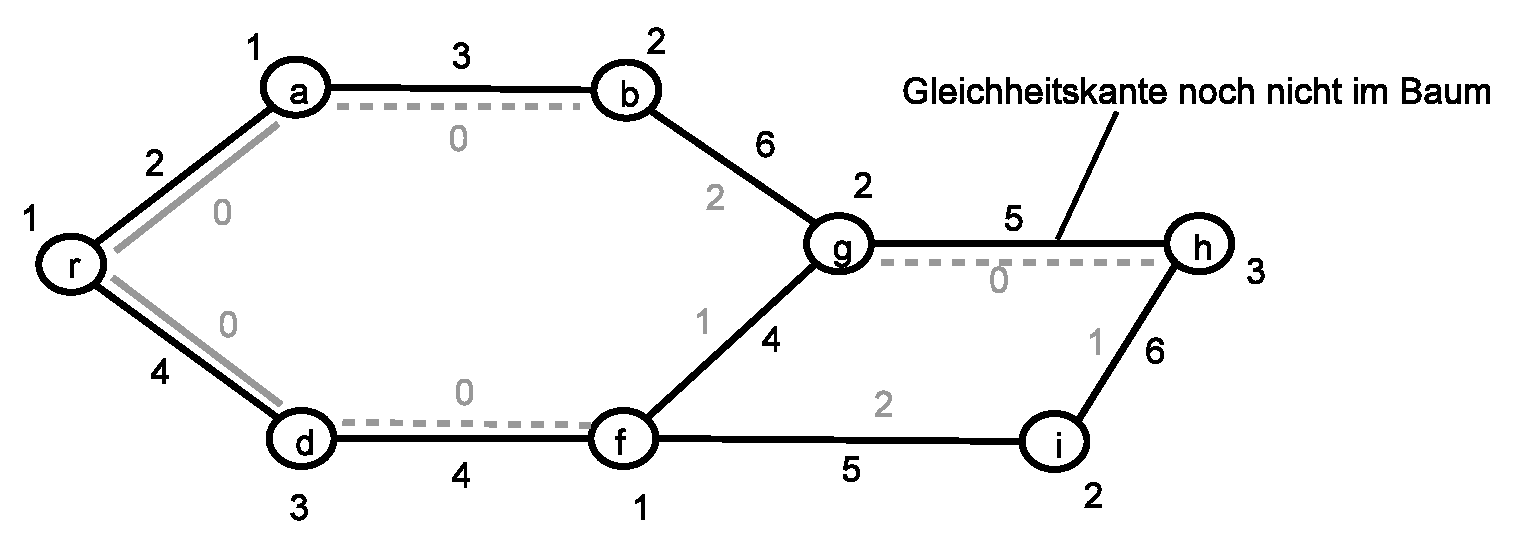
\includegraphics[height=2.3cm]{bilder/5-3StartMax}

Die grauen Kanten sind die Kanten des Baumes und die grauen Zahlen sind die
jeweiligen reduzierten Kosten.

$\exists$ perf. Matching, aber kein perf. Matching in $G_{=}$

\paragraph{Verändere $y$} \mbox{} \\
($M$ und $T$ sollen in $E_{=}$ bleiben, $\bc_e$ soll kleiner werden für
Kanten mit einem Knoten $\in B(T)$ und dem anderen $\not\in
B(T)$)
\begin{algorithmic}
\STATE Erhöhe $y_{v} \leftarrow y_v + \epsilon \; \; \forall v \in B(T)$
\STATE Erniedrige $y_v \leftarrow y_v - \epsilon \; \; \forall v \in A(T)$
\STATE Wähle $\epsilon > 0$ maximal unter:
\[y_u + y_v \leqq c_{u v} \; \; (\bc_{u v} \geqq 0)\]
\end{algorithmic}
Ergebnis: neue Kante, mit einem Knoten $\in B(T)$, der andere $\not\in
A(T)$ in $E_{=}$.\\
$G$ ist bipartit $\Rightarrow v \not\in V(T) \rightarrow$
Augmentierung/Baumerweiterung möglich. Im Beispiel $\epsilon =1$ aufgrund
der Kante $f g$.

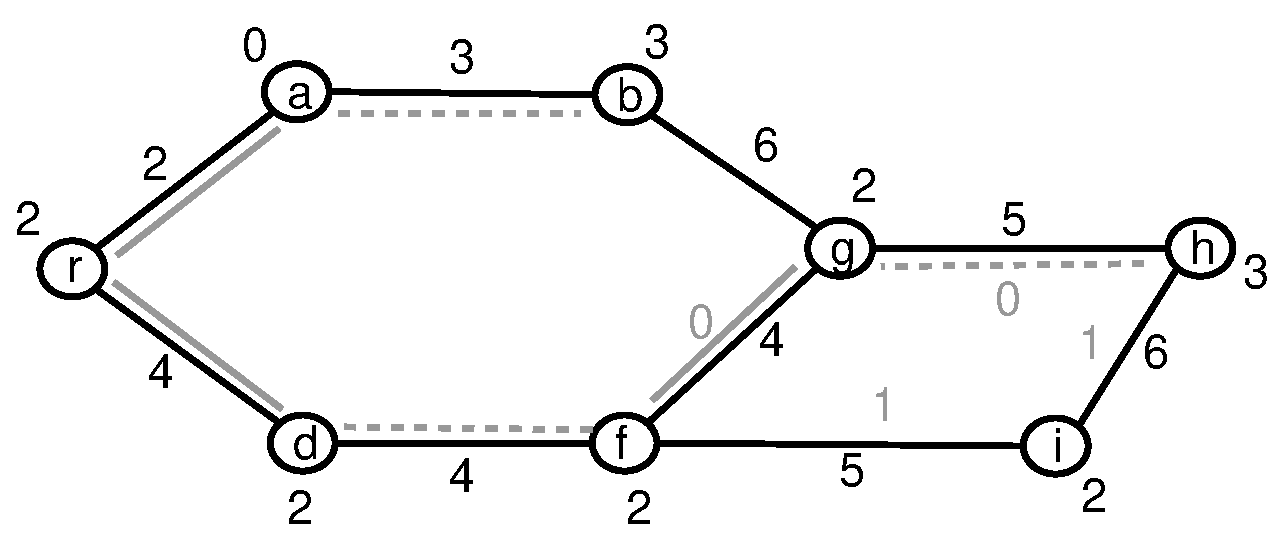
\includegraphics[height=2.3cm]{bilder/5-3StartMax2}

Daraufhin ergibt sich wieder $\epsilon = 1$:

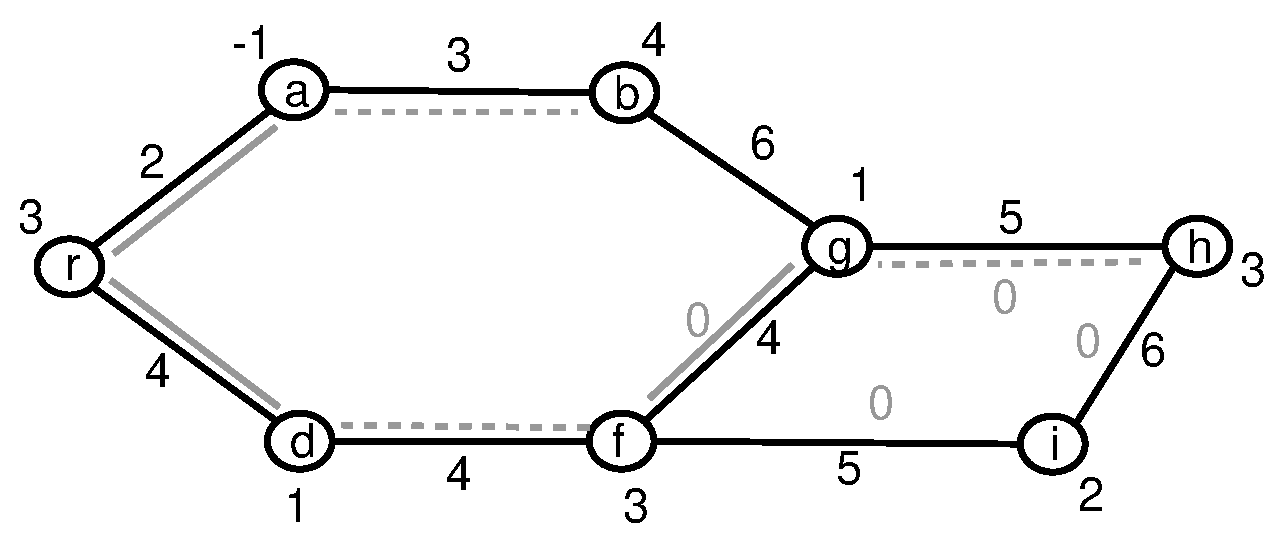
\includegraphics[height=2.3cm]{bilder/5-3StartMax3}

Diesmal haben wir zwei Möglichkeiten zu Augmentieren, entweder $h c$ oder
$f c$, je nachdem welche wir wählen ergeben sich zwei verschiedene
Matchings minimalen Gewichts.

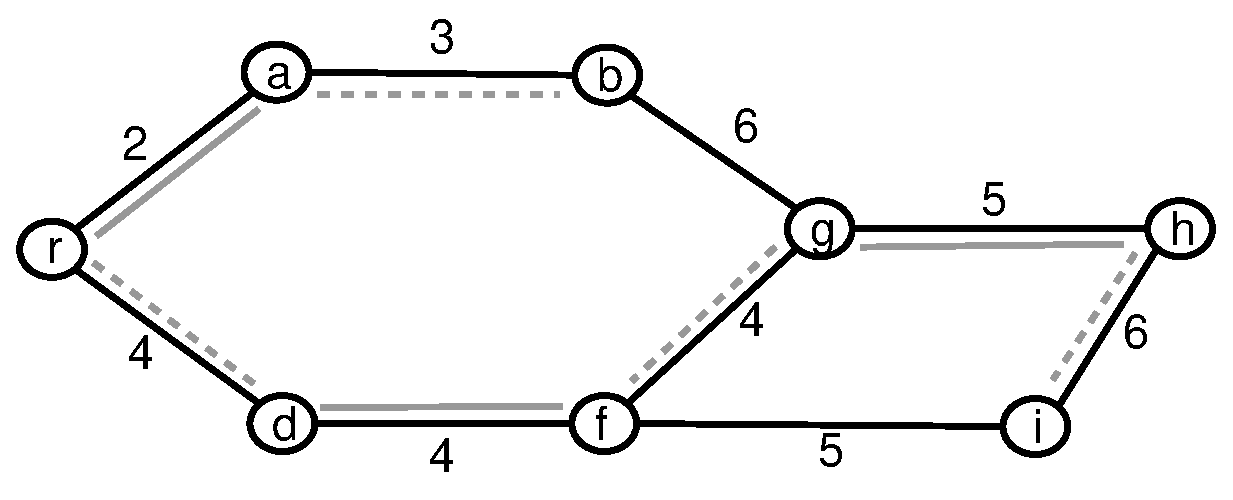
\includegraphics[height=2.3cm]{bilder/5-3StartMax4_1} \hspace{5mm}
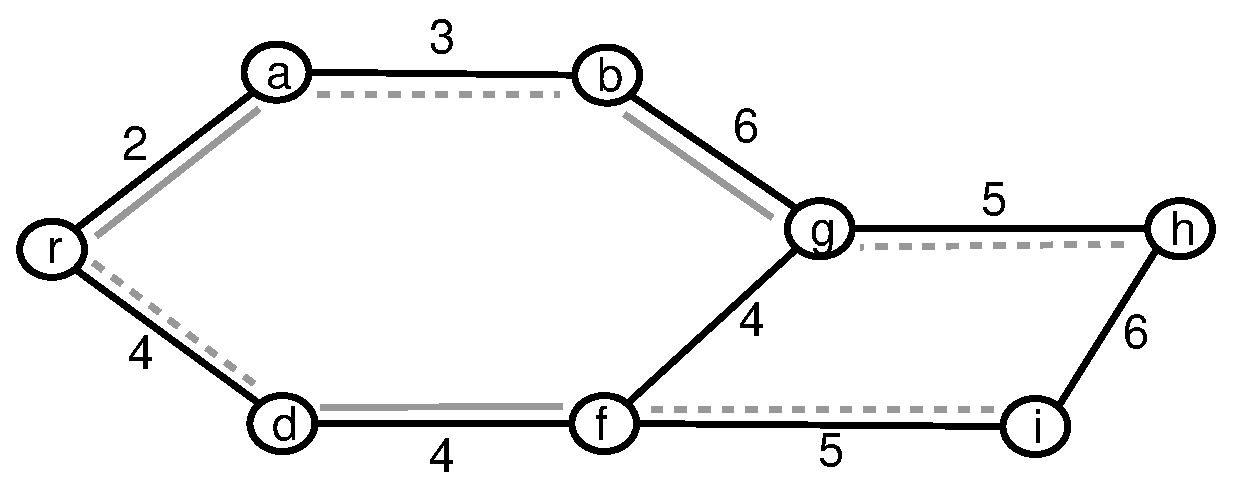
\includegraphics[height=2.3cm]{bilder/5-3StartMax4_2}

\subsubsection{Minimum Kosten perf. Matching Algorithmus für bipartite
Graphen}
(auch bekannt unter dem Namen "`Ungarische Methode"' [Kuhn 1955])\\
Eingabe: Graph $G$
\begin{algorithmic}
\STATE Sei $y$ zulässig für ($DLPPMMG'$), $M$ ein Matching in $G_{=}$;
\IF{$M$ ist perfekt}
\STATE STOP "`Matching $M$ perfekt mit minimum Kosten"';
\ENDIF
\STATE $T\leftarrow (\{r\}, \varnothing)$ wobei $r$ $M$-exponiert ist;
\LOOP 
\WHILE{($\exists v w \in E_{=}$ mit $v \in B(T)$, $w \not\in V(T)$)}
\IF{($w$ ist $M$-exponiert)}
\STATE Benutze $v w$ zur $M$-Augmentierung;
\IF{($\nexists$ $M$-exponierter Knoten in $G$)}
\STATE STOP "`Matching $M$ perfekt mit minimum Kosten"';
\ELSE
\STATE $T\leftarrow (\{r\},\varnothing)$ wobei $r$ $M$-exponiert ist;
\ENDIF
\ELSE
\STATE Benutze $v w$ zur Baumerweiterung;
\ENDIF
\ENDWHILE
\IF{($\forall v w \in E$ mit $v \in B(T)$ gilt $w \in A(T)$)} 
\STATE STOP "`$G$ hat kein perfektes Matching"';
\ELSE
\STATE $\epsilon \leftarrow \min\{\bc_{vw} | v \in B(T), \; w \not\in
V(T)\}$;
\STATE \textbf{forall} $(v \in B(T)) \; \; y_v \leftarrow y_v + \epsilon$;
\STATE \textbf{forall} $(v \in A(T)) \; \; y_v \leftarrow y_v - \epsilon$;
\ENDIF
\ENDLOOP
\end{algorithmic}

Laufzeit:\\
Schlimmstenfalls eine Dualänderung pro Baumerweiterung, d.h. $O(n^2)$
Dualänderungen mit jeweils $O(m)$ Arbeit, insgesamt $O(n^2m)$ Zeit. Kann
verbessert werden zu $O(n \, S(n,m))$ Zeit.

Erstes zulässiges $y$ kann in Zeit $O(n^2)$ gefunden werden:
Sei ($V_1,\,V_2$) Bipartition von $G$.
\begin{algorithmic}
\STATE \textbf{forall} $(v \in V_1)$ $y_v \leftarrow \min \{c_{v w}| w \in
V_2\}$
\STATE \textbf{forall} $(w \in V_2)$ $y_w \leftarrow \min \{c_{v w}-y_v | v
\in V_1\}$ 
\end{algorithmic}
Dann gilt $\bc_{v w} = c_{v w} - y_v - y_w \geqq \rightarrow 0$ nach
Konstruktion.

\subsubsection{Allgemeiner Fall (nicht bipartit)}

Im allgemeinen Fall gilt Satz \ref{BipBirkoff} nicht, z.B.:

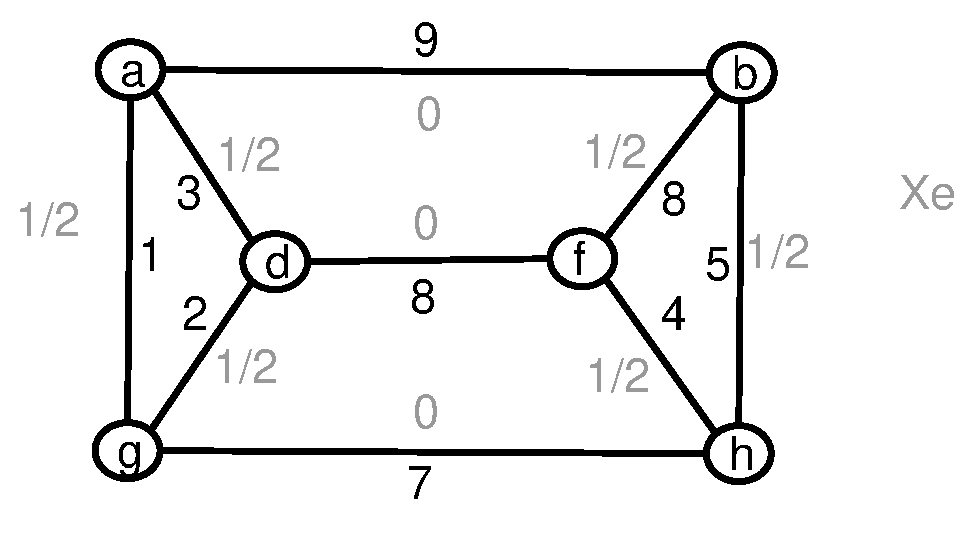
\includegraphics[height=2.5cm]{bilder/5-3Allg1}

Wert: $\displaystyle \sum_{e\in E} c_e x_e = \frac{1}{2}(1+2+3+4+5+6) =
10,5$

Aber: $\exists$ Minimum perf. Matching mit Kosten 14:

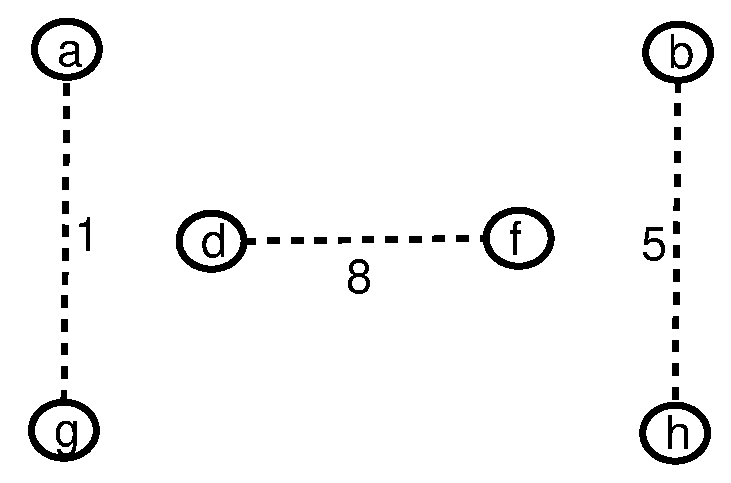
\includegraphics[height=2.5cm]{bilder/5-3Allg2}

\paragraph{Entwicklung einer besseren Schranke} (Edmonds[1965])\\
Schnitt $D= \delta(S)$ ungerade, falls |S| ungerade.

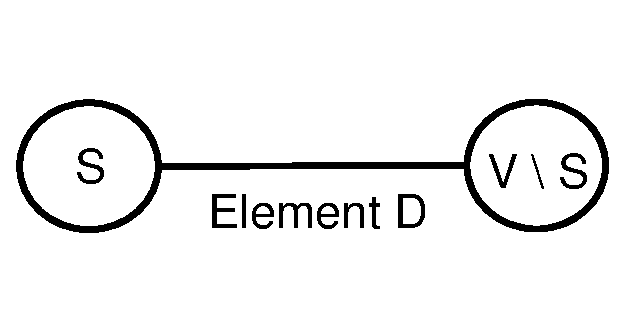
\includegraphics[height=1.2cm]{bilder/5-3Allg3}
 
In jedem perf. Matching $M$ existiert eine Kante aus $\delta(S)$\\
x Inzidenzvektor eines perf. Matchings in $G$.\\
$\Rightarrow$ ($\forall$ ungerade Schnitte $D$ in $G$) $x(D) \geqq 1$ 

Hinzufügen von $x(D) \geqq 1$ ergibt bessere Schranke. Im Beispiel wählen
wir $D=\{a b, d f, g h\}$ ergibt Optimalwert 14.

$\mathscr{C} =$ Menge aller ungeraden Schnitte, die nicht der Form
$\delta(v)$ für $v \in V$ sind.
\[\begin{array}{lrcll}
\mbox{(LPPMMG)} \hspace{5mm}&\multicolumn{4}{l}{\min \displaystyle \sum_{e \in E} c_e
x_e}\\
&x(\delta(v)) &=&1&\forall \; v \in V\\
&x(D) &\geqq&1&\forall \; D \in \mathscr{C} \\
&x_e&\geqq& 0&\forall \; e \in E
\end{array}
\]
Damit erhalten wir nicht nur eine bessere untere Schranke, sondern:
\begin{satz} \label{MatPolyEdmonds}
Matching Polytop Theorem von Edmonds [1965]

Sei $G=(V,E)$ ein Graph und $c \in R^E$. Dann hat $G$ ein perf. Matching
genau dann, wenn (LPPMMG) eine zulässige Lösung hat. Hat $G$ ein perf. Matching,
so ist das minimum Gewicht eines perf. Matchings in $G$ gleich dem
optimalen ZF-Wert von (LPPMMG) (vgl. Birkoff für bipartiten Fall)
\end{satz}
Beweis: Korrektheit durch folgenden Algorithmus. q.e.d.

\[\begin{array}{lrcll}
\mbox{(DLPPMMG)} \hspace{5mm}&\multicolumn{4}{l}{\max \displaystyle
\sum_{v\in V} y_v + \sum_{D \in \mathscr{C}} Y_D}\\
&y_v+y_w + \displaystyle \sum_{e\in D \in \mathscr{C}} Y_D
&\leqq&c_e&\forall \; e = v w \in E\\
&Y_D&\geqq&0&\forall \; D\in \mathscr{C}
\end{array}\]

Für $(y,Y)$ und $e \in E$:
\[\bc_e = \bc_e(y,Y) = c_e - y_v - y_w - \sum_{e \in D \in \mathscr{C}} Y_D\]
$(y,Y)$ zulässig für (DLPPMMG) $\Leftrightarrow \{ \begin{array}{l} Y_D \geqq
0 \; \; \forall \; D \in \mathscr{C}\\ \bc_e \geqq 0 \; \; \forall \; e \in
E\end{array}$

Komplementärer Schlupf:
\[\begin{array}{llcll}
\mbox{(KS)}&x_e > 0 & \Rightarrow&\bc_e = 0& (\forall \; e \in E)\\
&Y_D > 0&\Rightarrow x(D) = 1 & (\forall D \in \mathscr{C})
\end{array}
\]
$x$ Inzidenzvektor eines perf. Matchings:
\[
\mbox{(KS)} \Rightarrow \begin{array}{lcll} e \in M &\Rightarrow& \bc_e =
0&(\forall \; e \in E)\\
Y_D >0 &\Rightarrow |M \cap D| =1&(\forall\; D \in \mathscr{C})
\end{array} 
\]



$G'$ abgeleitet von $G$

$\Rightarrow$ Jeder ungerade Schnitt in $G'$ ist eine ungerader Schnitt in
$G$. D.h. jeder Schnitt der Form $\delta_{G'}(v)$ korrespondiert zu einem
ungeraden Schnitt in $G$. Nur solche erhalten positive $Y_D$. D.h.
Variablen $y_v$ reichen, hier $y_v \geqq 0$

Vorgehen analog zum bipartiten Fall.\\
$y$ Änderung: $\epsilon$ wie gehabt plus:
\[\epsilon \leqq \frac{1}{2} \bc_e \mbox{ für } e_{vw} \mbox{ mit }v,w \in
B(T)\]
Bei einer Gleichheitskante sind beide Endknoten $\in B(T)$\\
Also Schrumpfe Blüte:

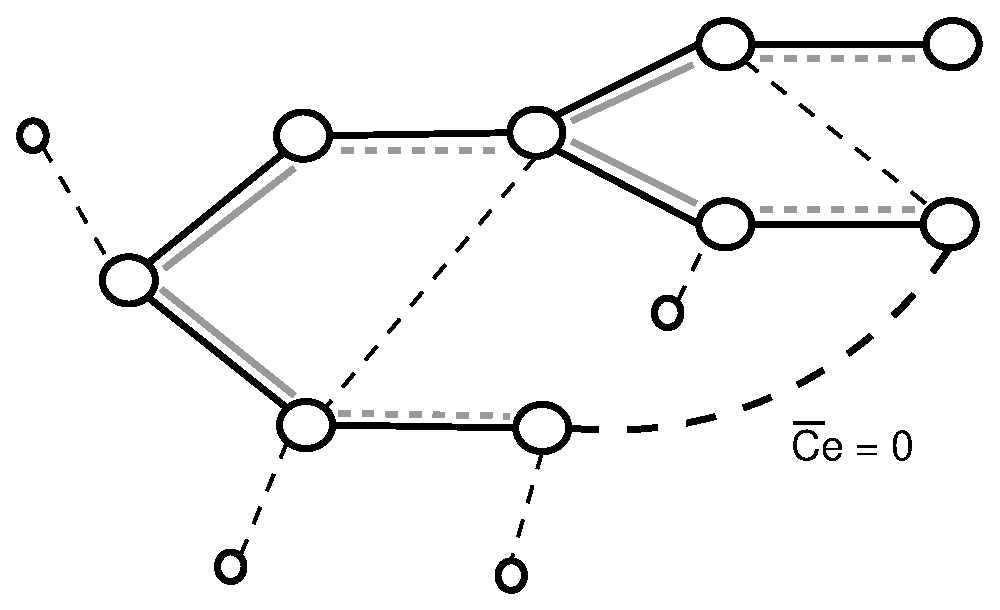
\includegraphics[height=2.5cm]{bilder/5-3SchrumpfAllg}

Komponente wird zu $c$ zusammengefasst:

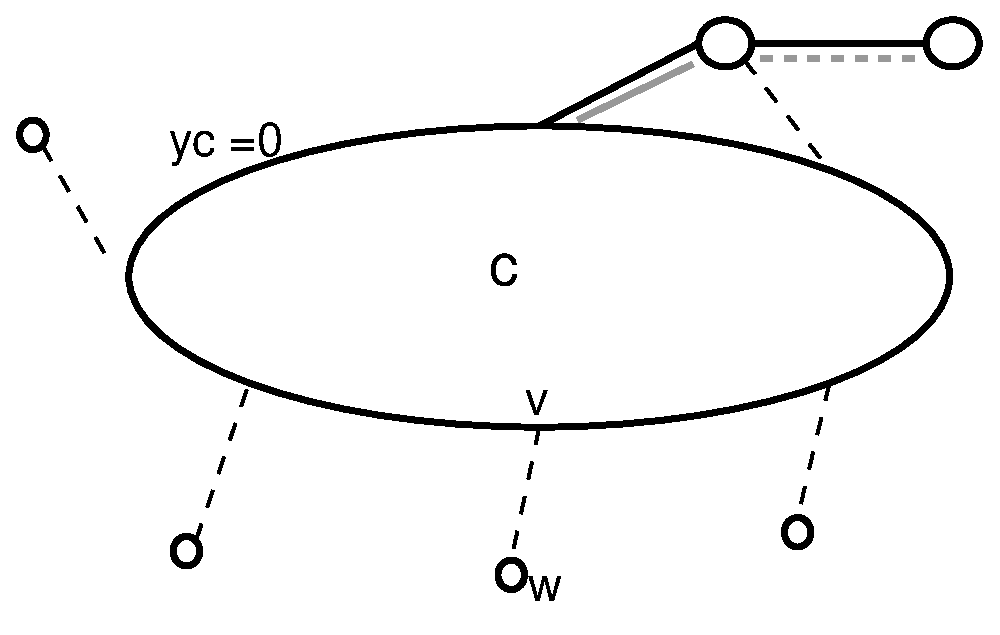
\includegraphics[height=2.5cm]{bilder/5-3SchrumpfAllg2}

Für alle $v w$ mit $v \in V(C)$ und $w \not \in V(C)$: $c'_{v w} 
\leftarrow c_{v w} -y_v$\\
Dies erhält die reduzierten Kosten auf allen übrig gebliebenen Kanten.
$(G,c) \rightarrow (G',c')$ ist "`abgeleitetes Paar"'.

\paragraph{Benutze $v w$ zum Schrumpfen und adaptiere $M'$ und $T$
(Neu)}\mbox{}\\
Eingaben:
\begin{itemize}
\item Matching $M'$ von $G'$
\item $M'$-alternierenden Baum $T$
\item $vw \in E(G')$ mit $v,w \in B(T)$
\end{itemize}
Sei $C$ der Kreis gebildet aus $v w$ und dem $(v,w)$-Weg in $T$

\begin{algorithmic}
\STATE $G' \leftarrow G' \times C$;
\STATE $M' \leftarrow M' \wout E(C)$;
\STATE \textbf{forall} ($s t \in E(G')$ mit $s \in V(C)$, $t \not \in V(C))$
$c'_{s t} \leftarrow c'_{s t} - y_s$;
\STATE $y_C \leftarrow 0$;
\end{algorithmic}
Beispiel:

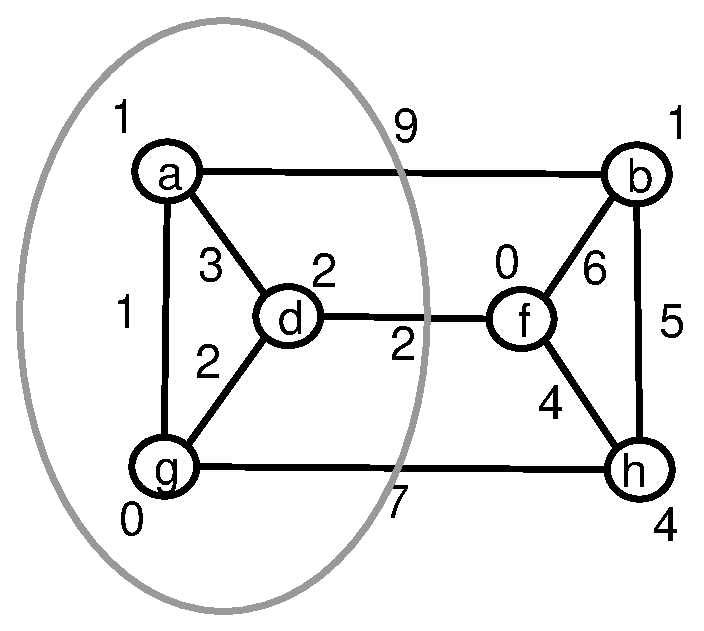
\includegraphics[height=3cm]{bilder/5-3vwSchrumpf}

ergibt:

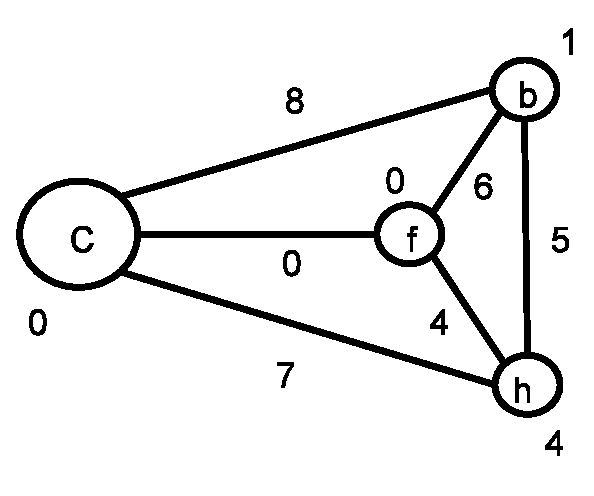
\includegraphics[height=2cm]{bilder/5-3vwSchrumpf2}

wobei ein perfektes Matching in der unteren Zeichnung einem perfekten
Matching in der oberen Zeichnung entspricht.

\begin{lemma} \label{DualSchrGleich}
$(G,c) \rightarrow (G',c')$ durch Schrumpfen eines ungeraden Kreises $C$
aus Gleichheitskanten bzgl. dual zulässiger Lösung. 
\end{lemma}

$M'$-perfektes Matching in $G'$:\\
$(y',Y')$ zulässig für (DLPPMMG) für ($G',c'$)\\
$(M',(y',Y'))$ erfülle (KS und $y'_c \geqq 0$)

$M$ ist perf. Matching in $G$ durch Erweiterung mit Kanten aus $E(C)$\\
Definiere $(y,Y)$:
\begin{itemize}
\item Schon definiert für $v \notin V(C)$
\item $y_v = y'_v$ für $v \in V \wout V(C)$
\item $Y_D = \left\{ \begin{array}{ll}Y'_D& \mbox{falls } Y'_D > 0\\
y'_C & \mbox{falls } D = \delta_{G'}(C)\\ 0&\mbox{sonst} \end{array}
\right\}$ für $D \in \mathscr{C}$
\end{itemize}

dann ist $(y,Y)$ zulässig für (DLPPMMG) für $(G,c)$ und $(M,(y,Y))$
erfüllen die KS-Bedingungen. q.e.d.

\subsubsection{Dualvariablenänderung}
Wie im bipartiten Fall:\\
plus $\epsilon \leqq  \frac{1}{2} c_e$ für Kanten mit beiden Endknoten in
$B(T)$\\
plus $\epsilon \leqq y_v$ für Pseudoknoten in $A(T)$

Beispiel:

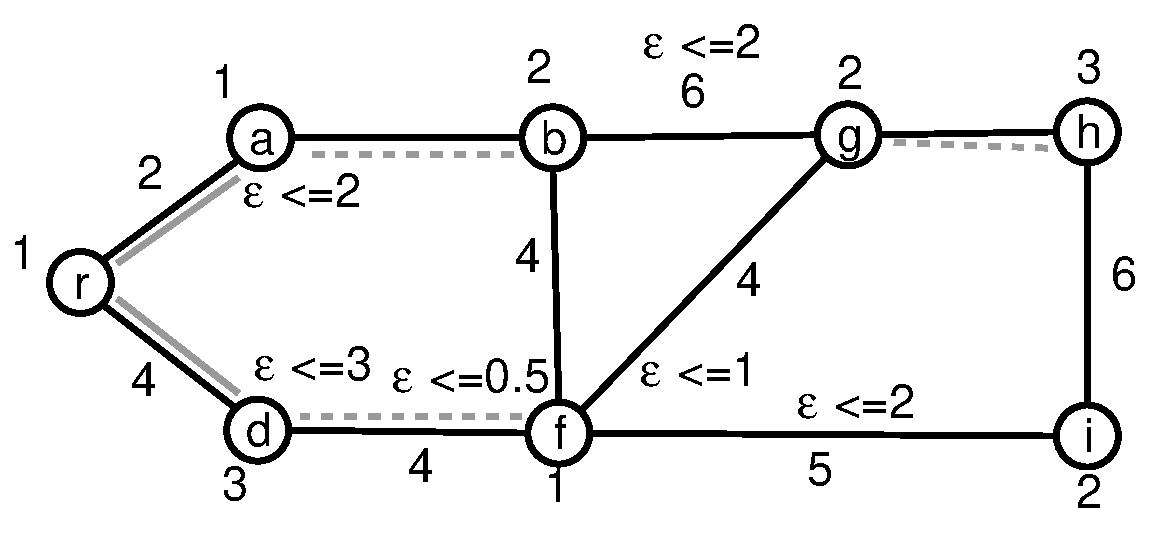
\includegraphics[height=2.3cm]{bilder/5-3Dual} 

(bei Dieser Zeichnung bin ich mir nicht sicher ob ich alles abgemalt
habe...)

$b f$ wird Gleichheitskante, danach Blütenschrumpfen.

\paragraph{Ändere $y$} \mbox{}\\
Eingaben:
\begin{itemize}
\item abgeleitetes Paar $(G',c')$
\item zulässige Lösung $y$ für (DLPPMMK) für $(G',c')$
\item Matching $M'$ von $G'$ aus Gleichheitskanten
\end{itemize}
\begin{algorithmic}
\STATE $\epsilon_{1} \leftarrow \min\{\bc_e | e =v w \in E(G'),\; v \in B(T), \;
w \not \in V(T)\}$;
\STATE $\epsilon_{2} \leftarrow \min\{ \frac{\bc_e}{2} | e = v w \in E(G'),
\; v \in B(T), \; w \in B(T)\}$;
\STATE $\epsilon_{3} \leftarrow \min\{y_v| v \in A(T), \; v \mbox{
Pseudoknoten in }G'\}$;
\STATE $\epsilon \leftarrow \min\{\epsilon_{1}, \epsilon_{2},
\epsilon_{3}\}$;
\STATE \textbf{forall} ($v \in B(T)$) $ y_v \leftarrow y_v + \epsilon$;
\STATE \textbf{forall} ($v \in A(T)$) $y_v \leftarrow y_v - \epsilon$;
\end{algorithmic}

Expandiere ungerade Pseudoknoten

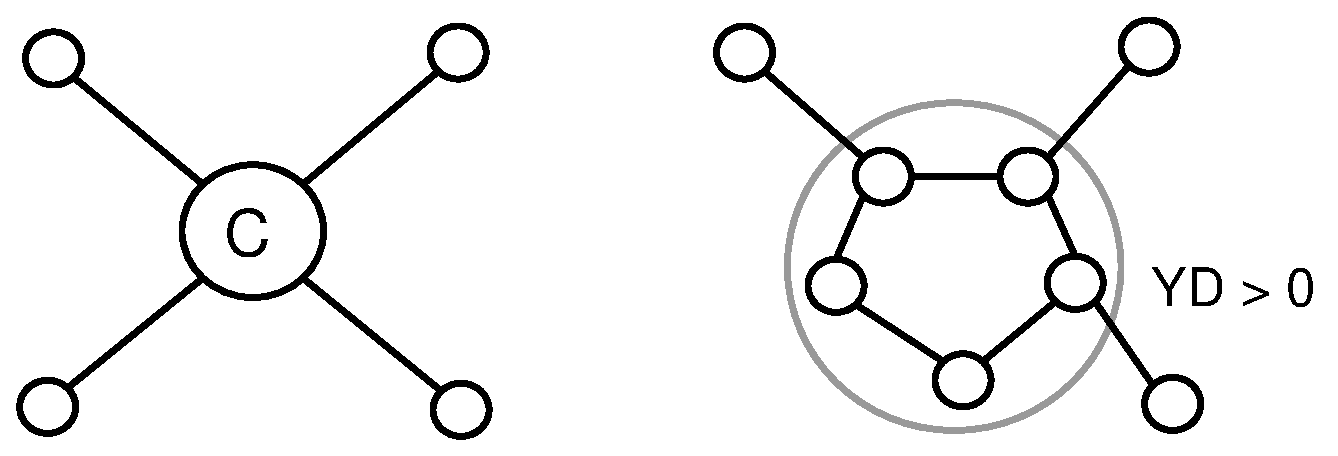
\includegraphics[height=2.3cm]{bilder/5-3Expand1}

Dies ist nicht von der Form $D = \delta_{G'}(v)$, also nur "`erlaubt wenn
$y_c = 0$. Wir müssen expandieren wenn $\epsilon_3$ "`greift'". Dann
entsteht keine neue Gleichheitskante zum Schrumpfen, Augmentieren, oder
Erweitern.

Wir sind dabei, einen Baum $T$ aufzubauen, deshalb außer adaptieren von
$M'$ und $c'$ auch Adaptieren von $T$.

Beispiel:


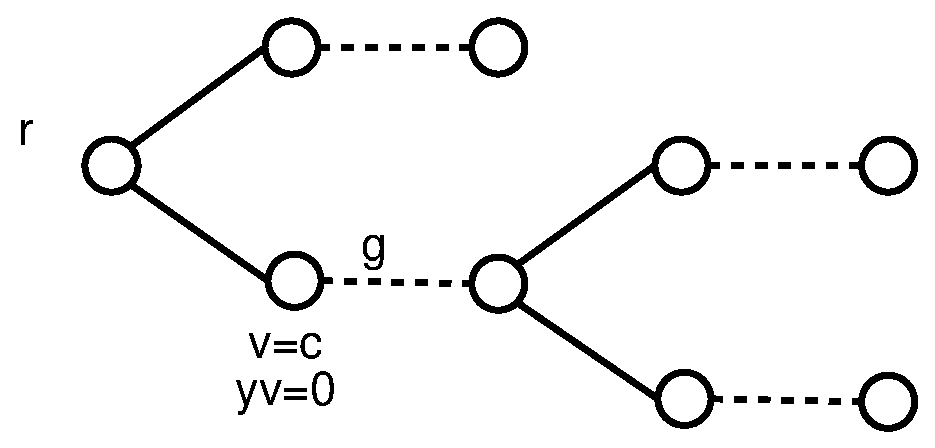
\includegraphics[height=2.3cm]{bilder/5-3Expand2}

\vspace{4mm}

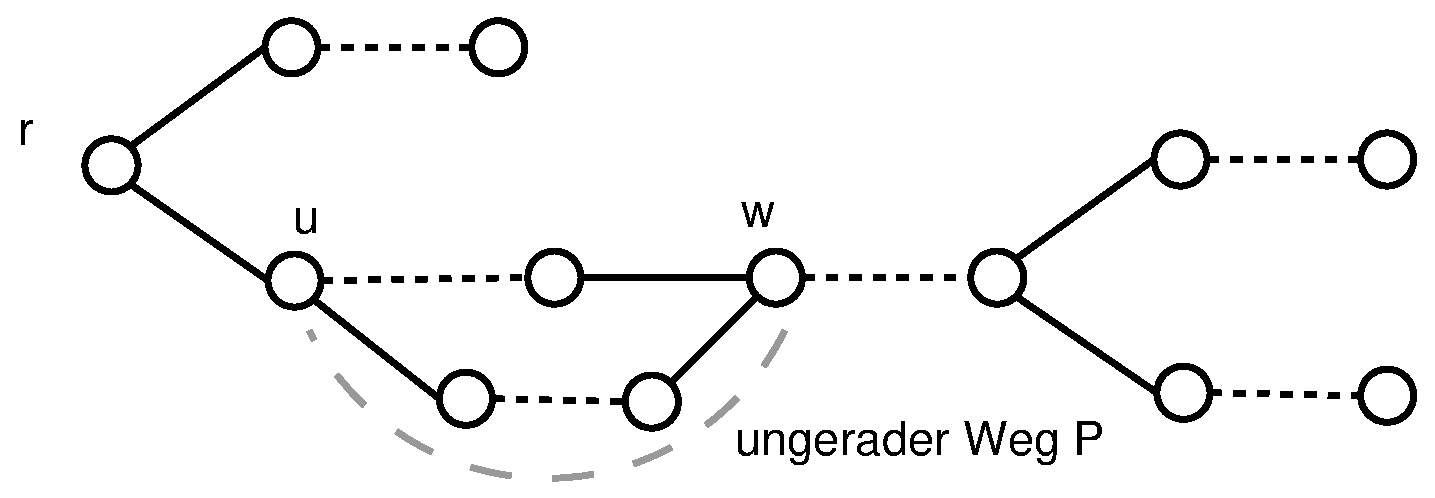
\includegraphics[height=2.5cm]{bilder/5-3Expand3}

\vspace{4mm}

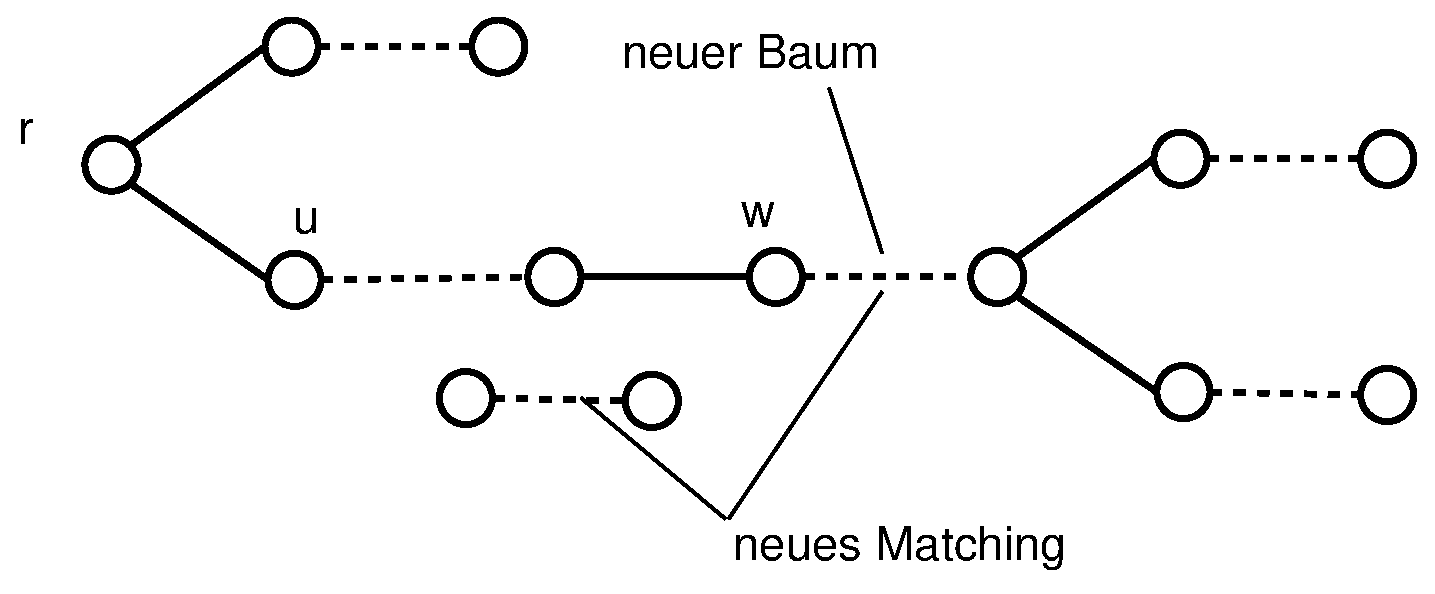
\includegraphics[height=3cm]{bilder/5-3Expand4}

\paragraph{Expandiere Pseudoknoten $v$ und adaptiere $M', T,c'$} \mbox{}\\
Eingaben:
\begin{itemize}
\item Matching $M'$ aus Gleichheitskanten in abgeleitetem Graphen $G'$
\item $M'$-alternierender Baum $T$ aus Gleichheitskanten
\item Pseudoknoten $v$ in $G'$ mit $y_v = 0$
\end{itemize}

\begin{algorithmic}
\STATE Ersetze $G'$ und $T$ durch Expandierung von $C$;
\STATE (Neuer Baum $T$ hat Kantenmenge $E(T) \wout E(P)$.)
\STATE Ersetze $M'$ durch expandiertes Matching;
\STATE \textbf{forall} ($s t \in E(G')$ mit $s \in V(C)$, $t \not \in
V(C)$) $c'_{s t} \leftarrow c'_{s t} + y_s$;

\end{algorithmic}

\begin{lemma}
Nach Anwendung des Expansions Unterprogramms ist $M'$ ein Matching in
$E_{=}$ und $T$ ein $M'$-alternierender Baum aus Gleichheitskanten. q.e.d.
\end{lemma}

\paragraph{Blüten-Schrumpf Algorithmus für perfektes Matching mit minimum
Kosten}\mbox{}\\
Eingabe: Graph $G$:
\begin{algorithmic}
\STATE Sei $y$ zulässig für (DLPPMMG), $M'$ ein Matching in $G_{=}$,
$G'=G$;
\IF{($M'$ ist perfekt)}
\STATE STOP "`Matching $M'$ perfekt mit minimum Kosten"';
\ENDIF
\STATE $T \leftarrow (\{r\},\varnothing)$ wobei $r$ $M'$-exponiert in $G'$
ist;
\LOOP
\CASE{($\exists \; v w \in E_{=}(G'),\; v \in B(T), \; w \not \in V(T)$
$M'$-exponiert)}
\STATE Benutze $v w$ zur $M'$-Augmentierung;
\IF{($\nexists \; M'$-exponierter Knoten in $G'$)}
\STATE Erweitere $M'$ zu perfektem Matching $M$ in $G$;
\STATE STOP "`Matching $M$ perfekt mit minimum Kosten"';
\ELSE
\STATE $T\leftarrow (\{r\},\varnothing)$ wobei $r$ $M'$-exponiert ist;
\ENDIF
\ENDCASE
\CASE{($\exists v w \in E_{=}(G')$ mit $v \in B(T)$, $w \not \in V(T)$
$M'$ überdeckt)}
\STATE Benutze $v w$ zur Baumerweiterung;
\ENDCASE
\CASE{($\exists v w \in E_{=}(G')$ mit $v \in B(T)$, $w \in B(T)$)}
\STATE Benutze $v w$ zum Schrumpfen und adaptiere $M'$, $T$, $c'$;
\ENDCASE
\CASE{($\exists$ Pseudoknoten $v \in A(T)$ mit $y_v = 0$)}
\STATE Expandiere $v$ und adaptiere $M'$, $T$,$c'$;
\ENDCASE
\CASE{(nichts von Obigem)}
\IF{($\forall v w \in E$ mit $v \in B(T)$ gilt $w \in A(T)$)}
\STATE STOP "`$G$ hat kein perfektes Matching"';
\ELSE 
\STATE Ändere $y$;
\ENDIF
\ENDCASE
\ENDLOOP
\end{algorithmic}

\begin{satz}
Der obige Algorithmus terminiert nach $O(n)$ Augmentierungen und $O(n^2)$
Baumerweiterungsschritten, $O(n^2)$ Expandierungsschritten und $O(n^2)$
Dualen Änderungsschritten.

Er berechnet ein perf. Matching mit minimum Gewicht oder stellt korrekt
fest, dass $G$ kein perfektes Matching hat.
\end{satz}
Beweis:\\
$O(n)$ Augmentierungsschritte. klar.

Wir zeigen $O(n)$ andere Schritte beim Aufbauen eines einzelnen Baums
$T$:\\
Nach jeder dualen Änderung folgt einer der anderen Schritte. Diese Zählen
wir:\\
Schrumpfen erzeugt einen neuen geraden "`$B$"'-Knoten in $T$. Expandiert
werden ungerade Pseudoknoten ("`$A$-knoten"').

Wir betrachten:
\[\begin{array}{rcl}
S_A &=& \displaystyle \sum_{v \in A(T),\; v \mbox{\scriptsize
 Pseudokn.}}|S(v)|\\
S_B &=& \displaystyle \sum_{v \in B(T), \; v \mbox{\scriptsize
 Pseudokn.}}|S(v)|\\
S_0 &=& \displaystyle \sum_{v \notin V(T), \; v \mbox{\scriptsize
 Pseudokn.}}|S(v)|\\
S=S_a - S_0
\end{array}\]
Expansion vermindert $S$\\
Schrumpfen und Baumerw. erhöhen $S$ nicht\\
$\Rightarrow O(n)$ Expandierungen

Schrumpfen erhöht $S_B$. Die anderen Schritte erniedrigen $S_B$ nicht.\\
$\Rightarrow O(n)$ Schrumpfungen

Baumerweiterung erhöht $|E(T)|$ um 2. Erniedrigung von $|E(T)|$ durch
Schrumpfen ist insgesamt höchstens $n$. Expandierung erniedrigt
$|E(T)|$ nicht.\\
$\Rightarrow O(n)$ Baumerweiterungen.

Terminierung "`$G$ hat kein perfektes Matching"': Korrektheit, Beweis wie
im ungerichteten Fall.

Terminierung mit perfektem Matching. Korrekt nach Lemma \ref{DualSchrGleich}
q.e.d.

Im Beweis von Satz \ref{MatPolyEdmonds} (Edmonds) fehlt jetzt nur noch:\\
$\not\exists$ perf. Matching $\Leftrightarrow$ (LPPMMG) hat keine zul.
Lösung.\\
"`$\Leftarrow$"' klar\\
"`$\Rightarrow$"' man zeigt: $\nexists$ perfektes Matching $\Rightarrow$
DLPPMMG ist unbeschränkt. q.e.d.

\begin{satz}
(Gabow [1990])\\
Es gibt eine Implementierung des Blütenschrumpf Algorithmus mit Laufzeit
$O(n m + n^2 \log n)$.
\end{satz}

\subsubsection{Optimale Duallösungen von Matchingproblemen}

\begin{satz}
Hat (DLPPMMG) eine Optimallösung, so auch eine verschachtelte, d.h. für
$s_1, s_2 \in \mathscr{S} = \{s \subseteq V| Y_{\delta(S)} > 0\}$ gilt
entweder $S_1 \cap S_2 = \varnothing$ oder $S_1 \subseteq S_2$ oder $S_2
\subseteq S_1$.\\
\end{satz}
Beweis: $y_v>0$ im Blütenschrumpf Algorithmus nur für Pseudoknoten in
Abgeleiteten Graphen.

\subsubsection{Dreiecksungleichung für die Gewichte}

\[c_{u v} + c_{v w} \geqq c_{u w} \; \; \forall \; u,v,w \in V\]

\begin{satz}
Sei $K_u = (V,E)$ ein vollständiger Graph auf $n$ Knoten, wobei $n$ gerade.
Sei $c \in \RR^E$, $c\geqq 0$ und $c$ erfülle die Dreiecksungleichung.

Startet der Blütenschrumpfalgorithmus mit $(y,Y)=0$, so gilt für die duale
Optimallösung bei Terminierung $y \geqq 0$.
\end{satz}
Beweis: Wir zeigen, dass $y$ während der Ausführung des Blütenschrumpf
Algorithmus nicht-negativ bleibt.\\
$y_v \leftarrow y_v - \epsilon \Rightarrow v$ ist ungerader "`$A$"'-Knoten
in $T$.

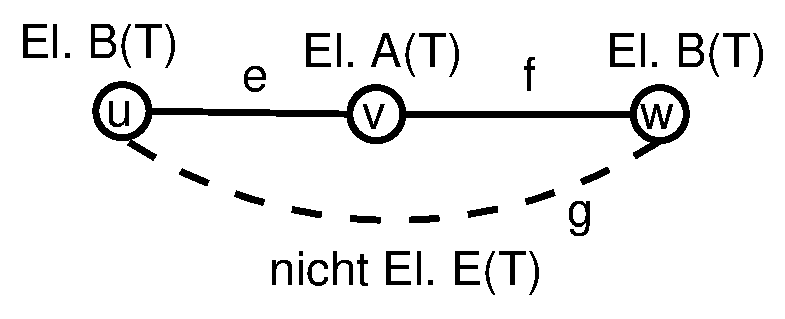
\includegraphics[width=5cm]{bilder/5-3VUngerKn}

Erweiterte Duallösung zu einer zulässigen Duallösung $(y,Y)$ im
Originalgraphen. Sei:
\[\begin{array}{rcl}
\mathscr{C}_e &=& \{D \in \mathscr{C} | Y_D > 0 \mbox{ und } e \in D\}\\
\mathscr{C}_f &=& \{D \in \mathscr{C} | Y_D > 0 \mbox{ und } f \in D\}\\
\mathscr{C}_g &=& \{D \in \mathscr{C} | Y_D > 0 \mbox{ und } g \in D\}
\end{array}\]
$\Rightarrow \mathscr{C}_g = \mathscr{C}_e \dot{\cup} \mathscr{C}_f$ wobei
$\dot{\cup}$ die disjunkte Vereinigung ist.

$\epsilon_0$ gilt $\epsilon \leqq \frac{1}{2} \bc_g$, also:
\[\begin{array}{rcl}
2 \epsilon &\leqq & \bc_g\\
&=& c_{u w} - y_u - y_w - Y(\mathscr{C}_g)\\
&\leqq& c_{u v} + c_{v w} - y_u - y_w - Y(\mathscr{C}_e) -
Y(\mathscr{C}_f)\\
&=& ( c_{u v} - y_u -Y(\mathscr{C}_e)) + (c_{v w} - y_w -
Y(\mathscr{C}_f))\\
&=& \bc_e + y_v + \bc_f + y_v\\
&\stackrel{\bc_e=\bc_f=0}{=} 2 y_v \Rightarrow \epsilon \leqq y_v
\hspace{4mm} y_v\mbox{ bleibt nicht-negativ}
\end{array}\]

Prima, jetzt können wir uns Zertifikate für die minimalen Matchings
(Zeichnungen mit den Kreisscheiben und Gräben, Kapitel 1) ausstellen, indem wir die
dualen Bedingungen dafür verwenden.

Mit dem Algorithmus rechnen wir nun die Radien der Kreisscheiben aus.
Ungerade Schnitte entsprechen ungeraden Knotenmengen. Gräben entstehen um
ungerade Knotenmengen. $y$ und $Y$ im Blütenschrumpfalgorithmus entsprechen
also genau den Kreisscheiben ($y$) bzw. Gräben ($Y$). Dies gilt aber nur
für euklidische Distanzen, bei der Max-Metrik wären es z.B. Quadrate.




